\documentclass[a4paper, 12pt]{report}

\usepackage[spanish]{babel}
\usepackage[utf8]{inputenc}
\usepackage[left=3cm, right=3cm, top=3cm, bottom=3cm]{geometry}
\usepackage{textcomp}
\usepackage{booktabs}
\usepackage{amssymb}
\usepackage{bussproofs}
\usepackage{fancyhdr}
\usepackage{graphicx}
\usepackage{amsmath}
\usepackage{enumitem}
\usepackage{ifsym}
\usepackage{float}


\usepackage{hyperref}
\hypersetup{
    colorlinks=true,
    linkcolor=blue,
    filecolor=magenta,
    urlcolor=cyan,
}

\pagestyle{fancy}
\lhead{Almeida, Figueroa, Ibarra \& Sánchez}
\chead{Tarea 6}
\rhead{\today}

\begin{document}
\begin{titlepage}
    \centering
    {\scshape\Huge Universidad Nacional Autónoma de México \par}
    \vspace{1.25cm}
    {\scshape\huge Fundamentos de Bases de Datos\par}
    \vspace{1.25cm}
    {\huge\bfseries Tarea 6:\\ Lenguaje de consulta SQL\par}
    \vspace{1.25cm}
    {\Large\textsc Almeida Rodríguez Jerónimo\par}
    \vspace{.1cm}
    {\large\texttt{418003815}\par}
    \vspace{0.25cm}
    {\Large\textsc Figueroa Sandoval Gerardo Emiliano\par}
    \vspace{.1cm}
    {\large\texttt{315241774}\par}
    \vspace{0.25cm}
    {\Large\textsc Ibarra Moreno Gisselle \par}
    \vspace{.1cm}
    {\large\texttt{315602193}\par}
    \vspace{0.25cm}
    {\Large\textsc Sánchez Lara Luis Enrique \par}
    \vspace{.1cm}
    {\large\texttt{418002856}\par}
    \vspace{1.5cm}
    \vfill
    \begin{figure}[hb!]
        
\includegraphics[width=.3\textwidth]
            {../../logos/escudo_f-ciencias.png}\hfill
        
\includegraphics[width=.3\textwidth]
            {../../logos/Escudo_UNAM.png}\hfill
    \end{figure}
\end{titlepage}
\subsection*{Instrucciones de uso}
% \begin{enumerate}
%     \item{\textt{Correr el SMBD de su preferencia}}
%     \item{\textt{}}
%     \item{\textt{}}
%
% \end{enumerate}

\subsection*{Consultas del inciso 4.}
\subsubsection*{Sub-inciso A}
\begin{figure}
    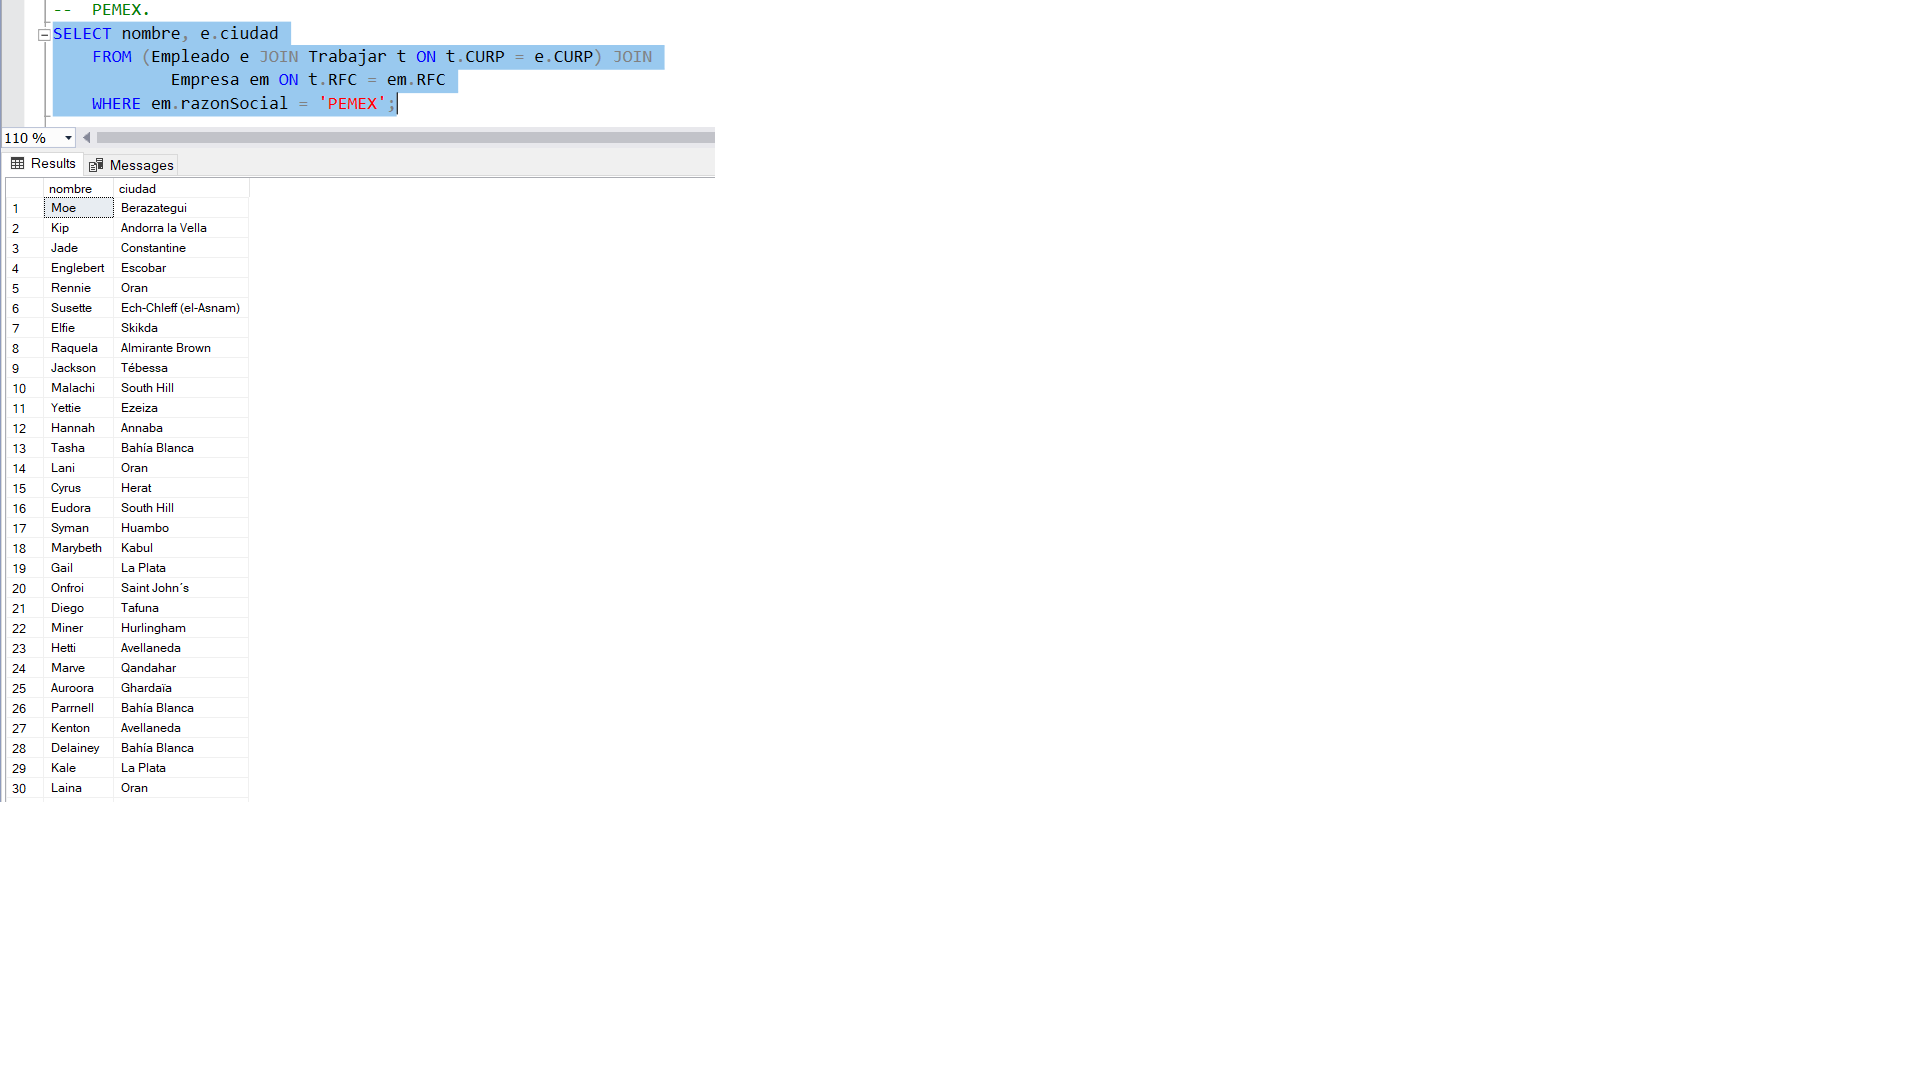
\includegraphics[width=\textwidth]
        {img/A1.png}\hfill
    \caption{A 1}
    \end{figure}
    \begin{figure}
        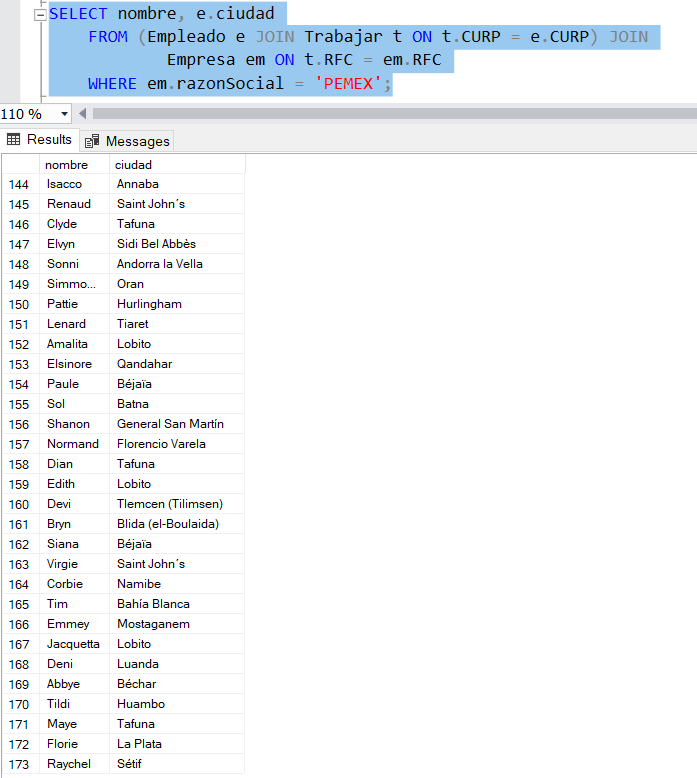
\includegraphics[width=\textwidth]
            {img/A2.png}\hfill
    \caption{A 2}
    \end{figure}

\subsubsection*{Sub-inciso B}
    \begin{figure}
        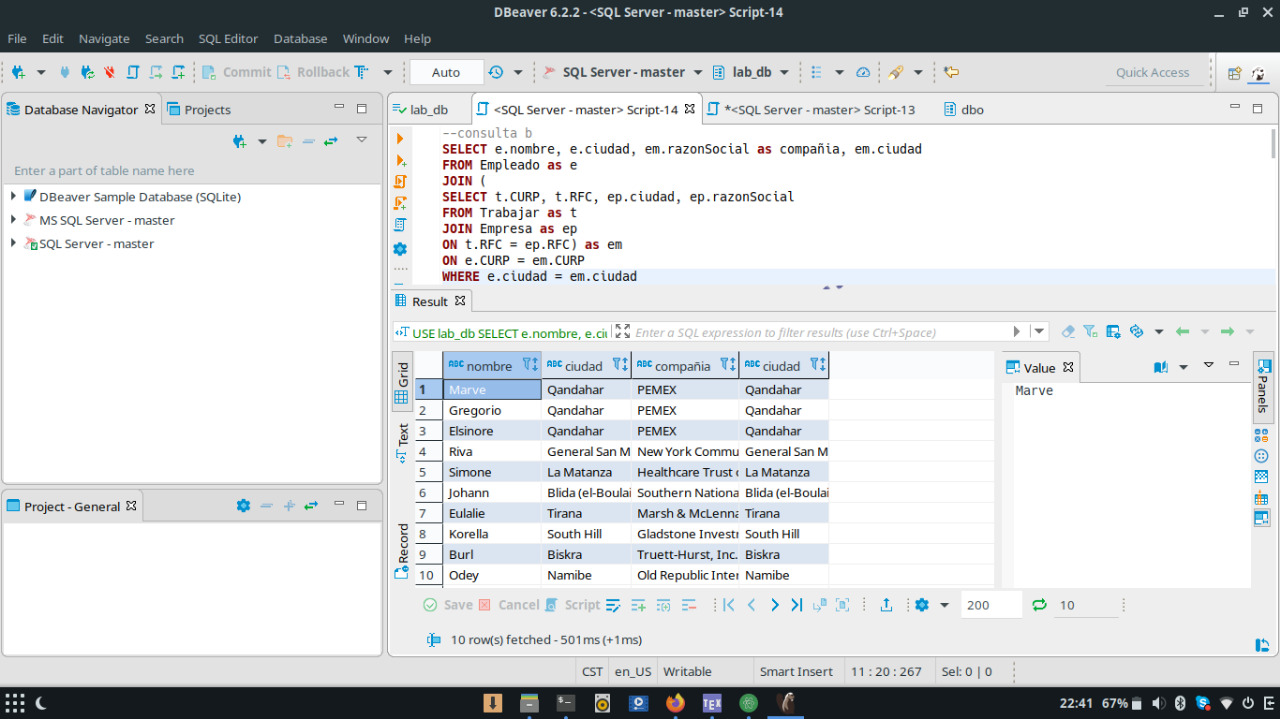
\includegraphics[width=\textwidth]
            {img/b1.jpeg}\hfill
        \caption{B}
    \end{figure}

\subsubsection*{Sub-inciso C}
    \begin{figure}
        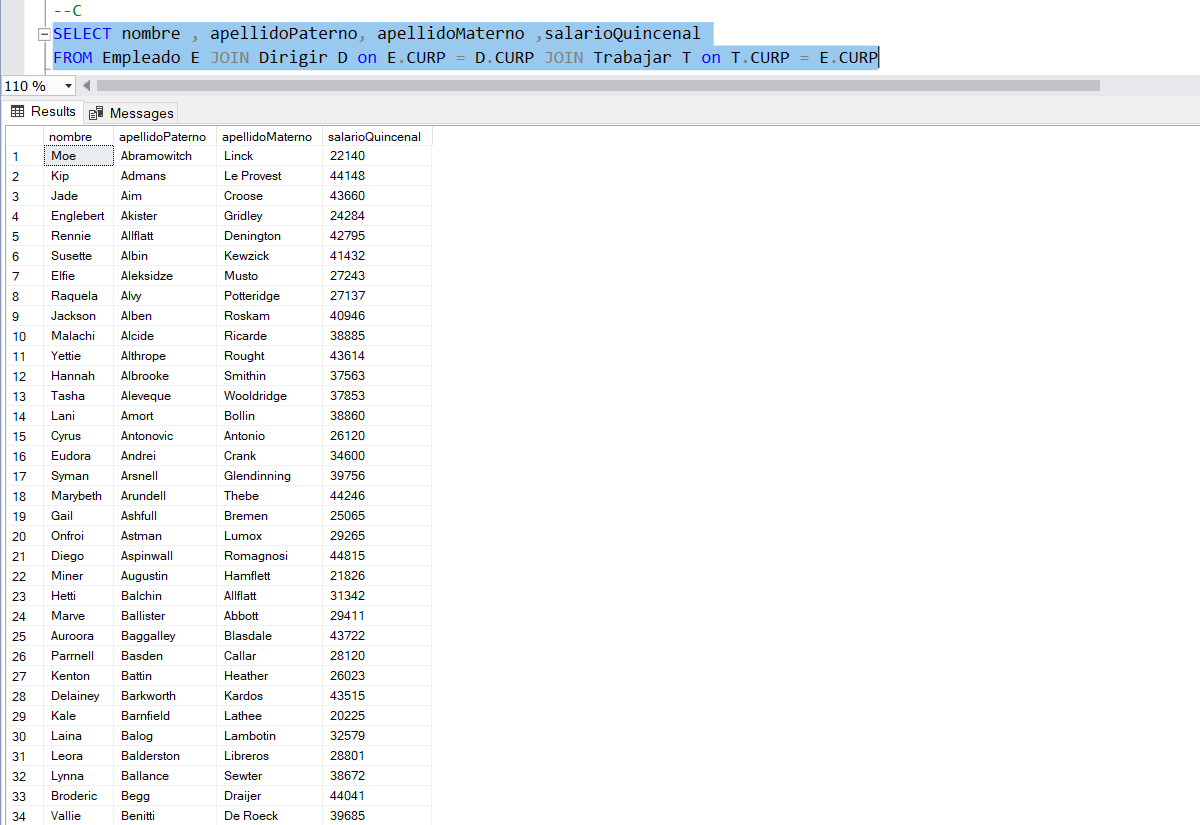
\includegraphics[width=\textwidth]
            {img/C1.png}\hfill
    \caption{C 1}
    \end{figure}
    \begin{figure}
        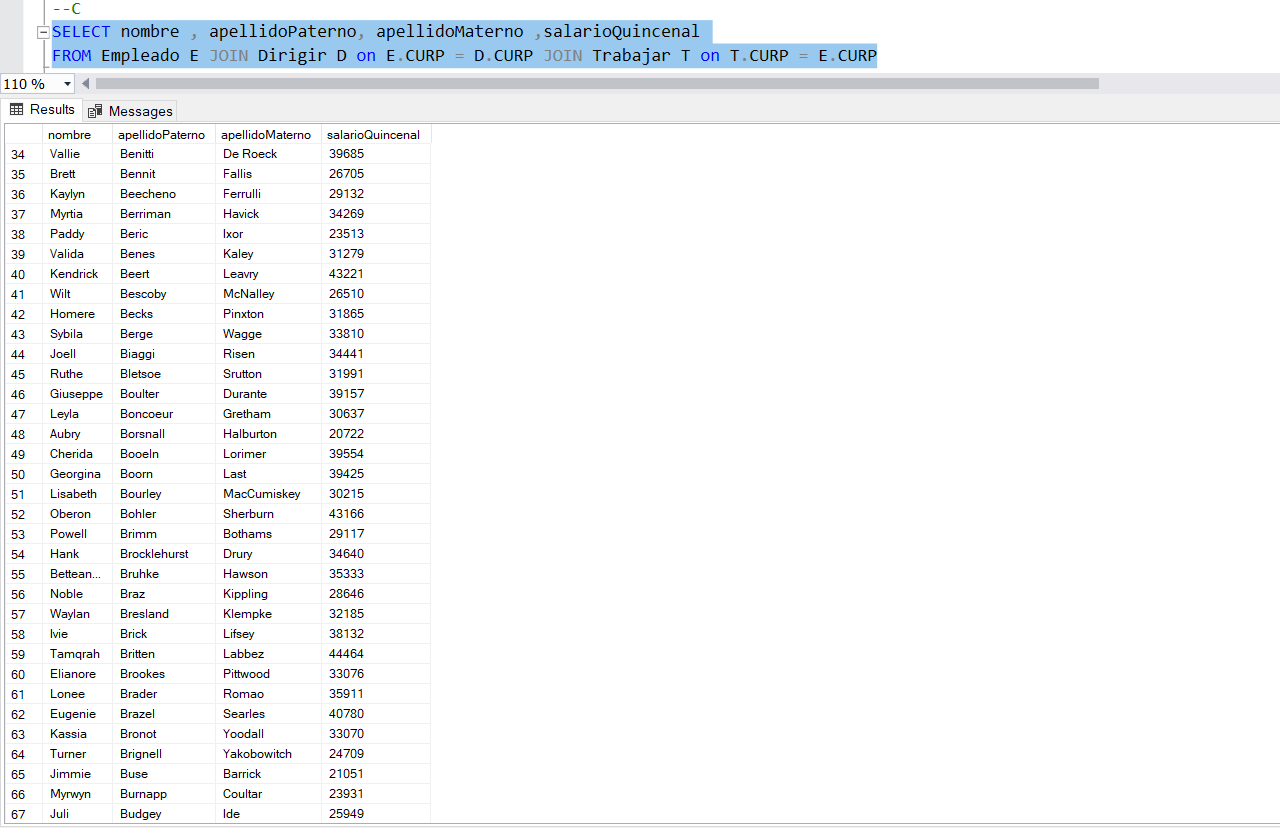
\includegraphics[width=\textwidth]
            {img/C2.png}\hfill
    \caption{C 2}
    \end{figure}
    \begin{figure}
        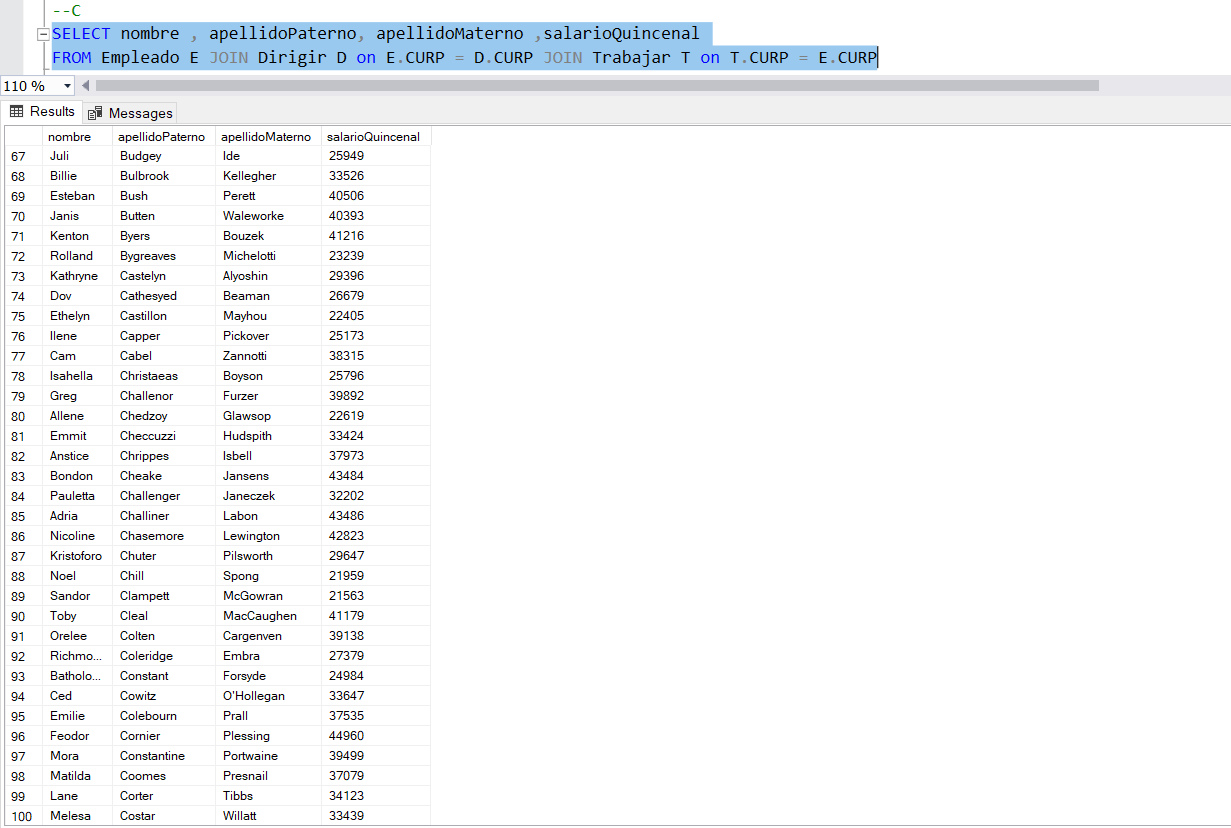
\includegraphics[width=\textwidth]
            {img/C3.png}\hfill
    \caption{C 3}
    \end{figure}
    \begin{figure}
        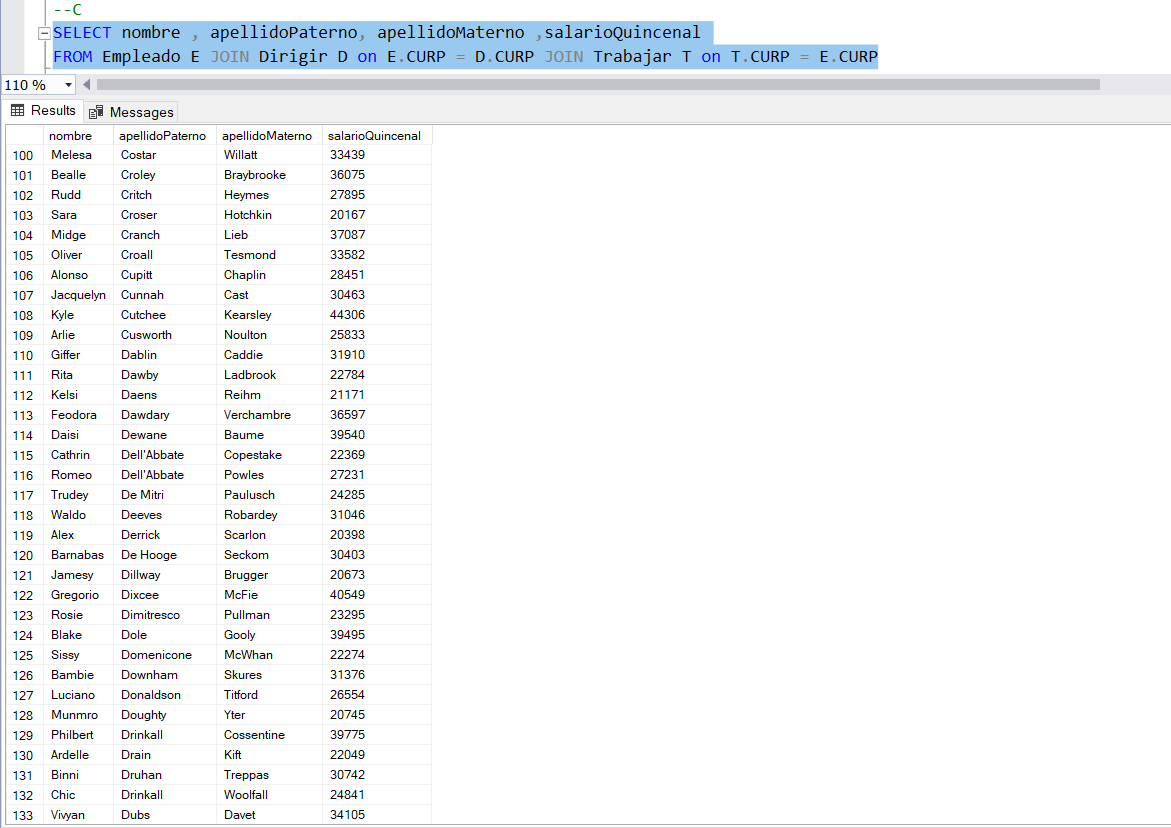
\includegraphics[width=\textwidth]
            {img/C4.png}\hfill
    \caption{C 4}
    \end{figure}
    \begin{figure}
        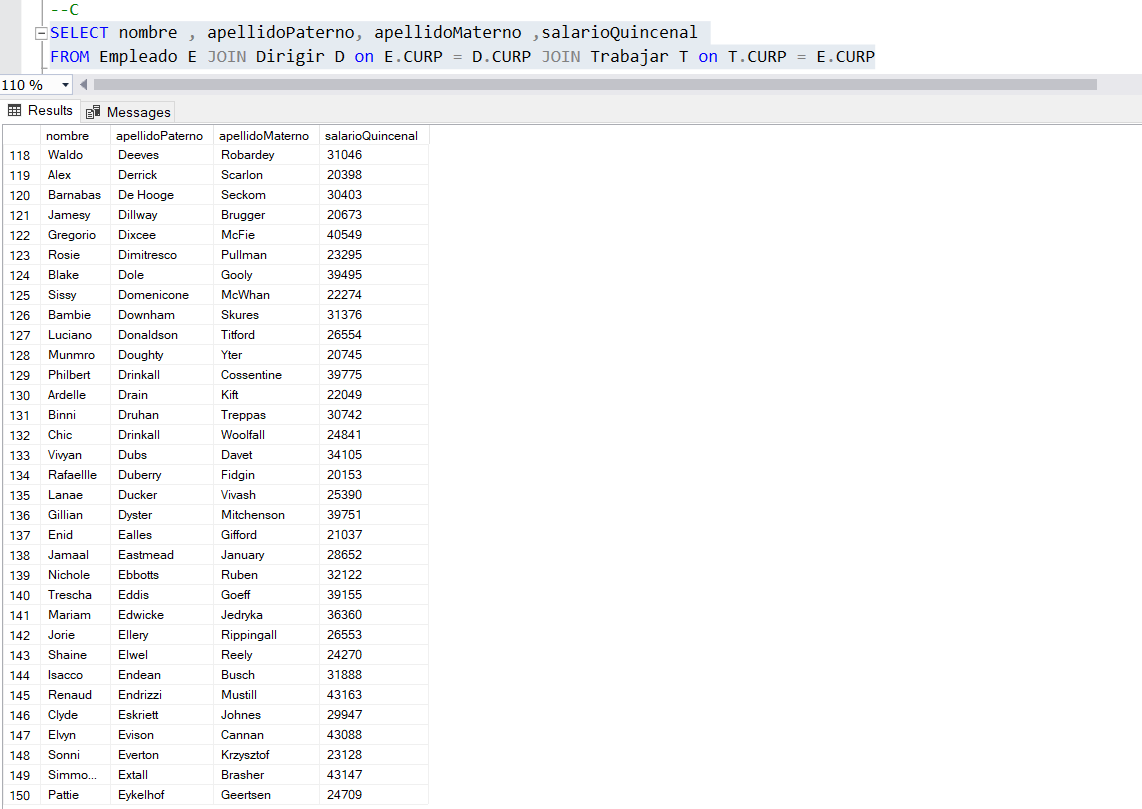
\includegraphics[width=\textwidth]
            {img/C5.png}\hfill
    \caption{C 5}
    \end{figure}

\subsubsection*{Sub-inciso D}
    \begin{figure}
        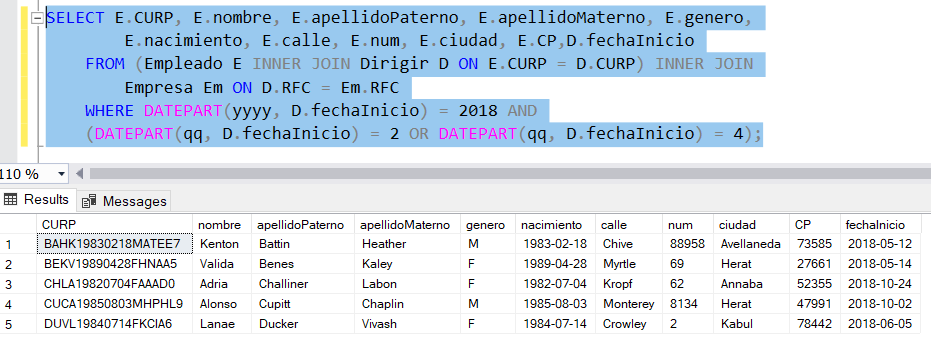
\includegraphics[width=\textwidth]
            {img/D.png}\hfill
    \caption{D}
    \end{figure}

\subsubsection*{Sub-inciso E}
    \begin{figure}
        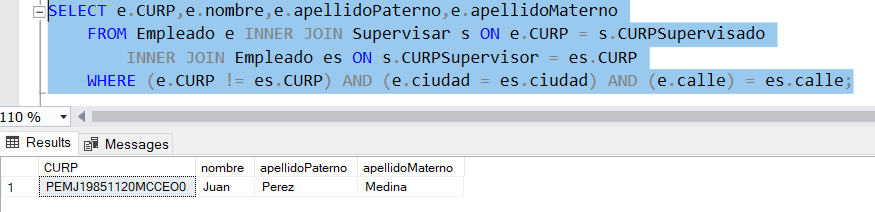
\includegraphics[width=\textwidth]
            {img/E.png}\hfill
    \caption{E}
    \end{figure}

\subsubsection*{Sub-inciso F}
    \begin{figure}
        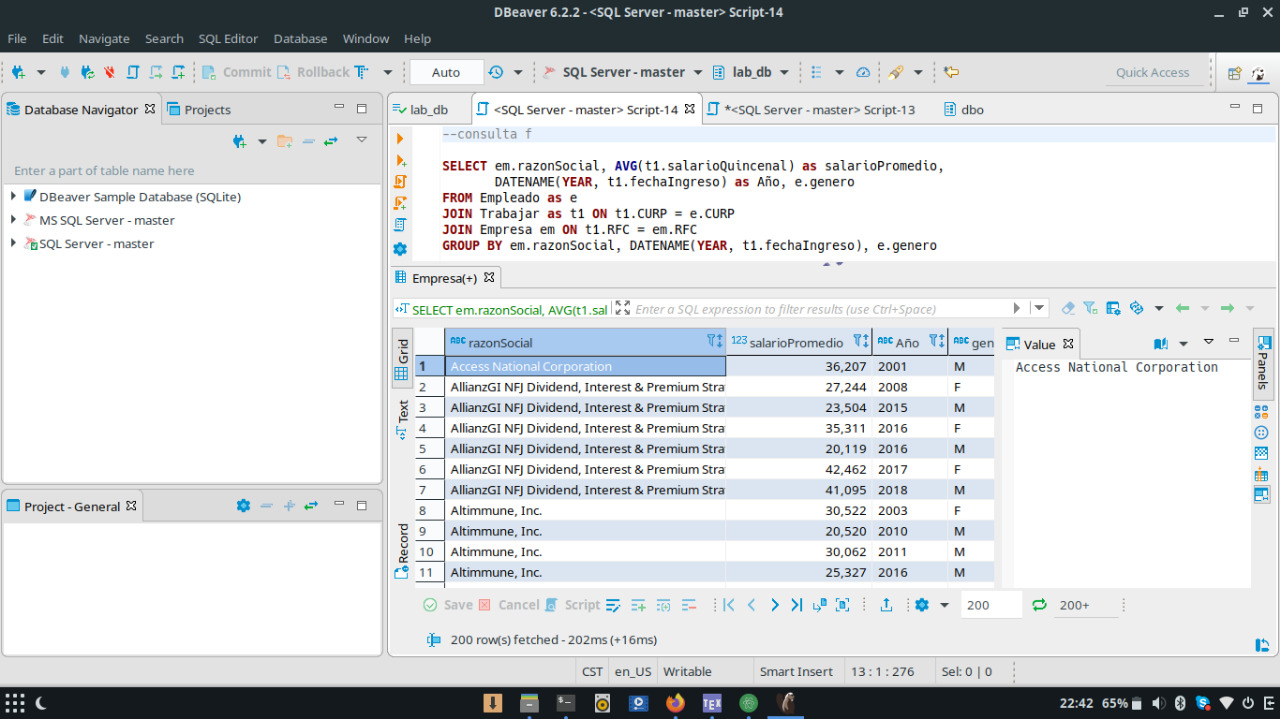
\includegraphics[width=\textwidth]
            {img/f1.jpeg}\hfill
    \caption{F 1}
    \end{figure}
    \begin{figure}
        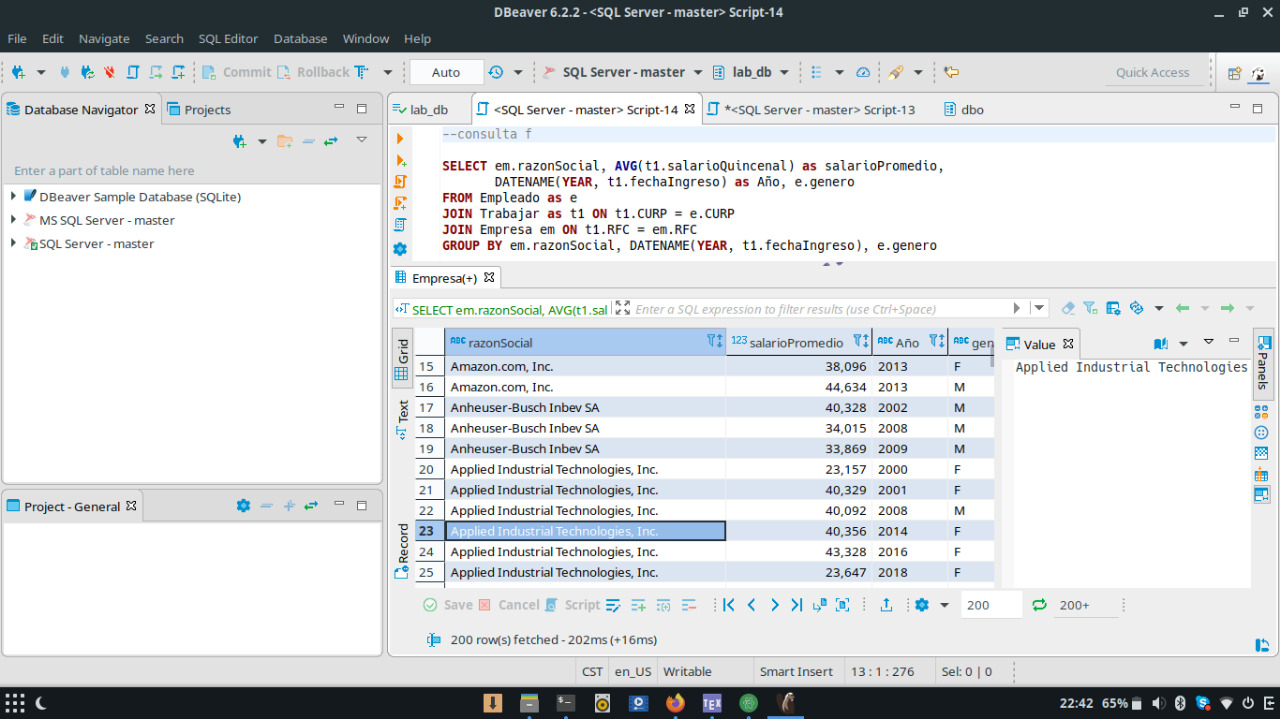
\includegraphics[width=\textwidth]
            {img/f2.jpeg}\hfill
    \caption{F 2}
    \end{figure}
    \begin{figure}
        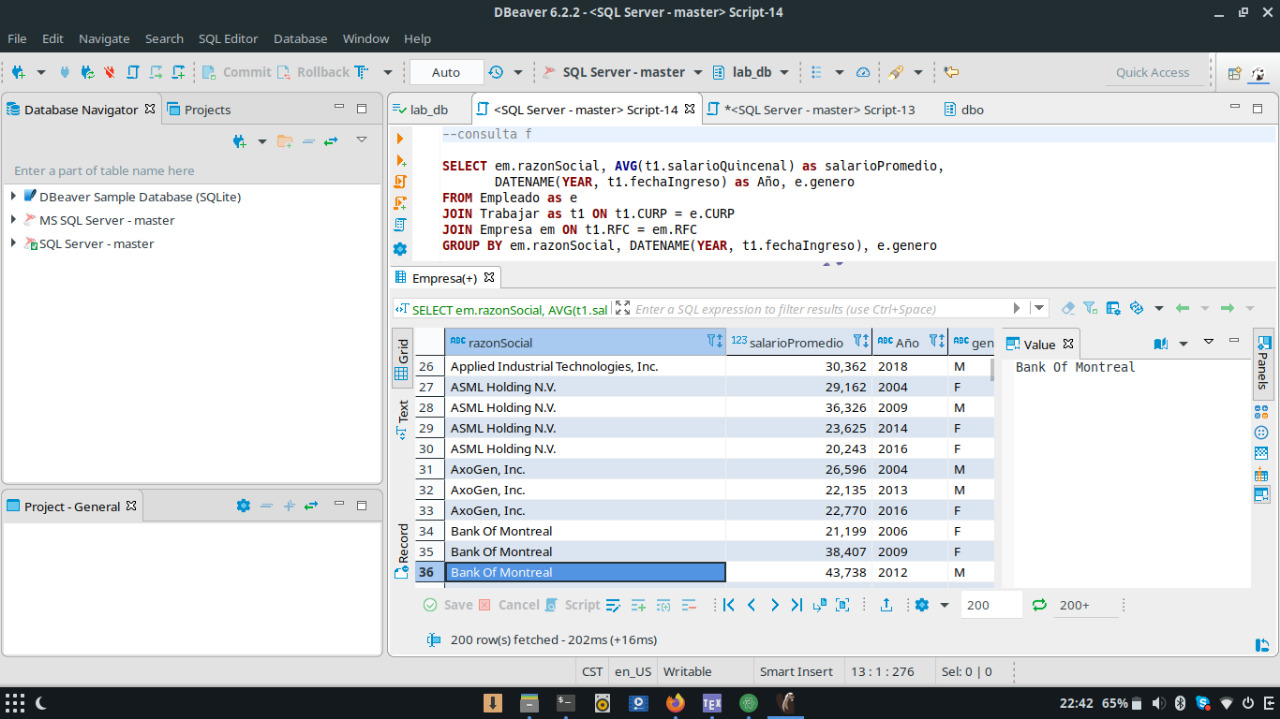
\includegraphics[width=\textwidth]
            {img/f3.jpeg}\hfill
    \caption{F 3}
    \end{figure}
    \begin{figure}
        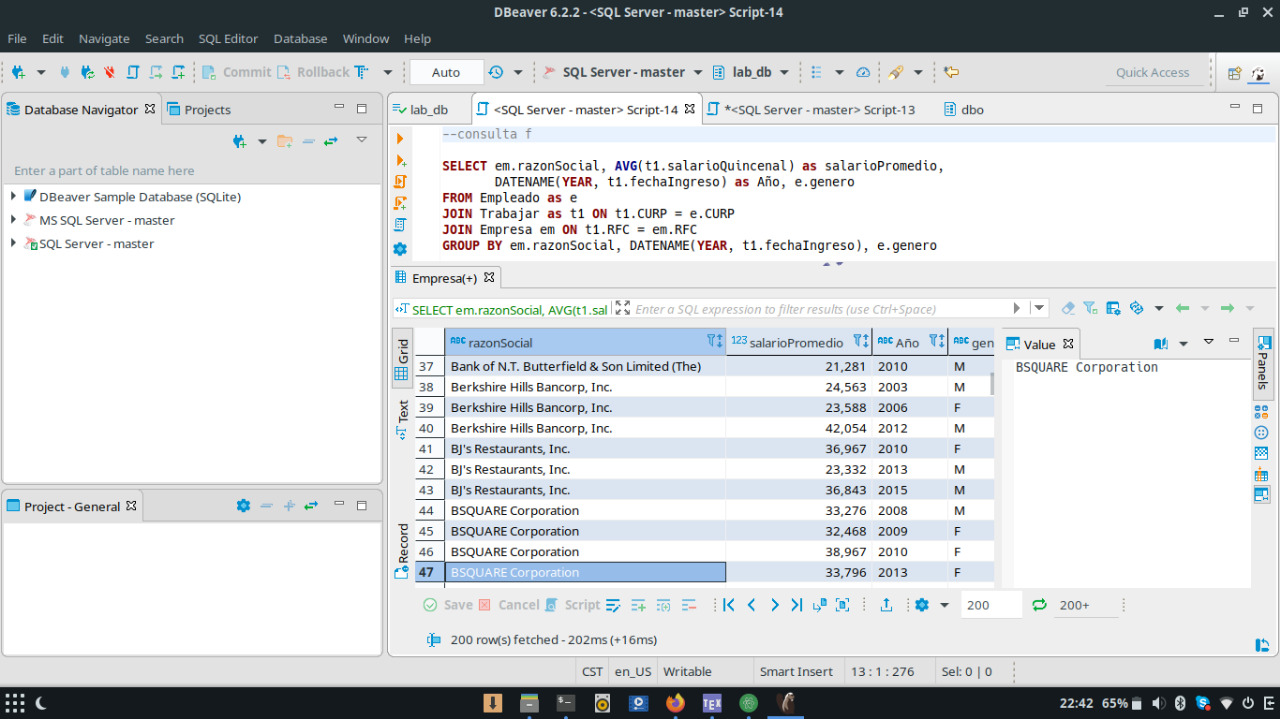
\includegraphics[width=\textwidth]
            {img/f4.jpeg}\hfill
    \caption{F 4}
    \end{figure}
    \begin{figure}
        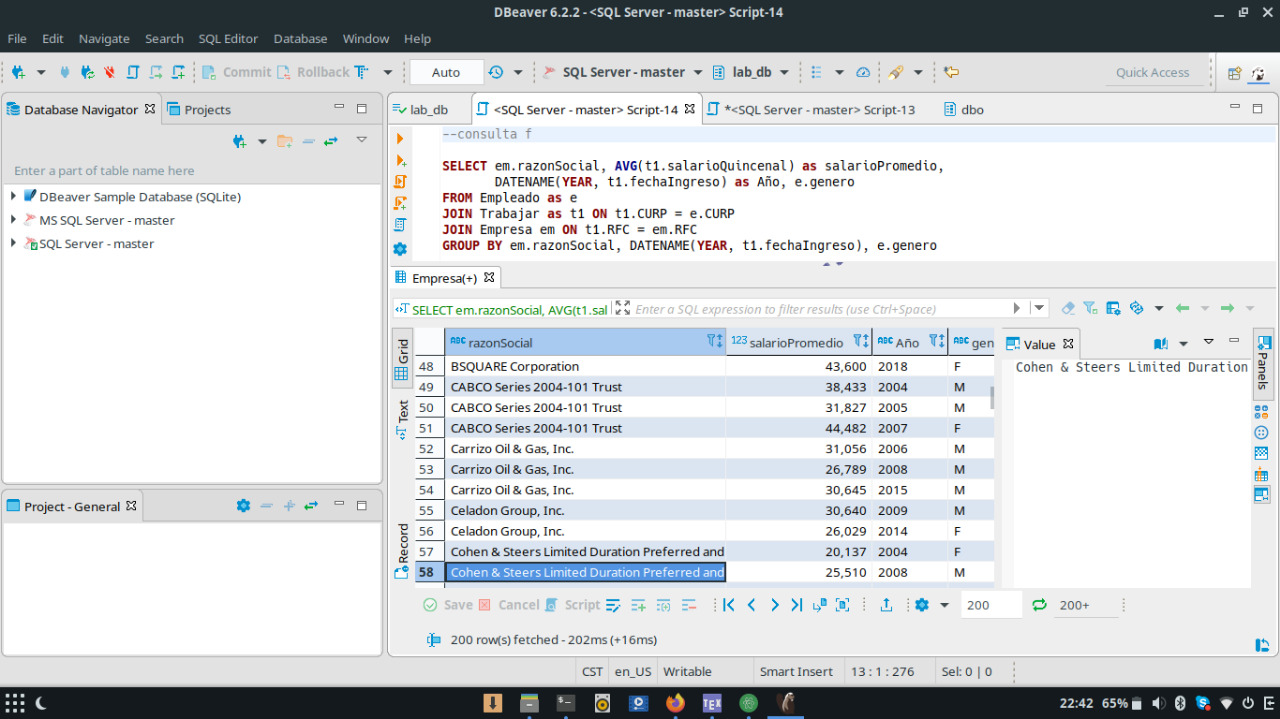
\includegraphics[width=\textwidth]
            {img/f5.jpeg}\hfill
    \caption{F 5}
    \end{figure}
    \begin{figure}
        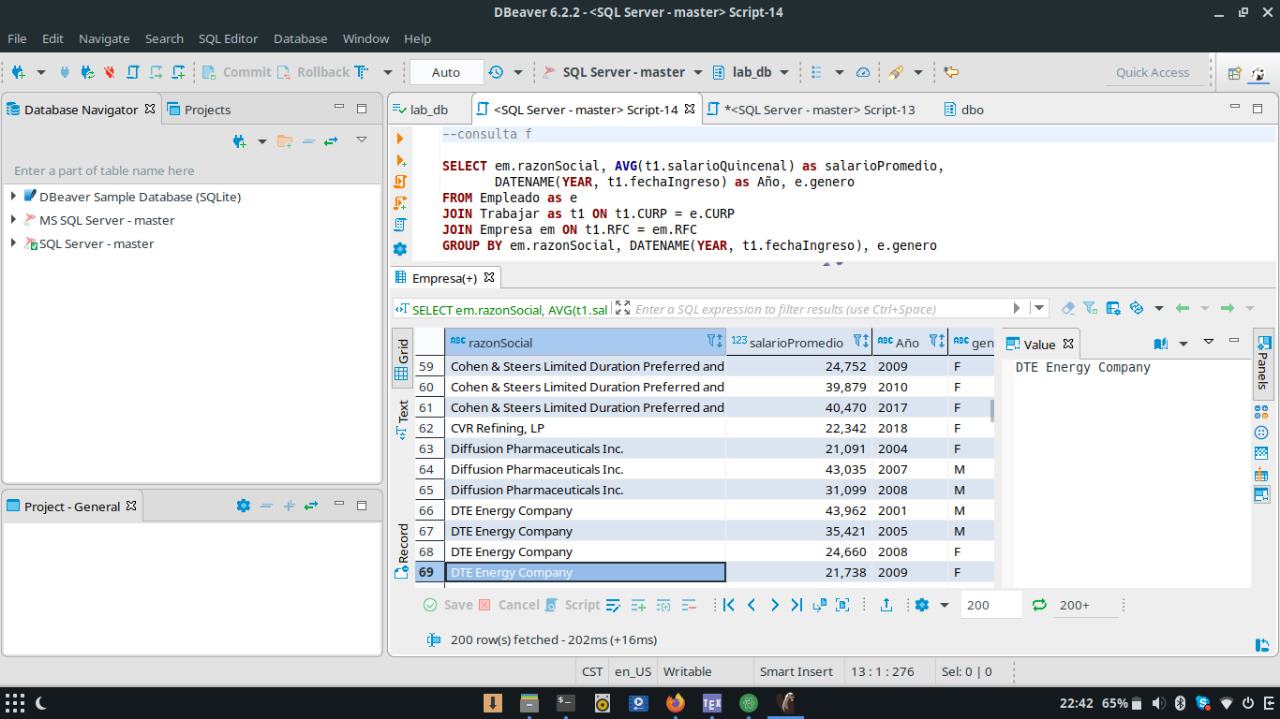
\includegraphics[width=\textwidth]
            {img/f6.jpeg}\hfill
    \caption{F 6}
    \end{figure}
    \begin{figure}
        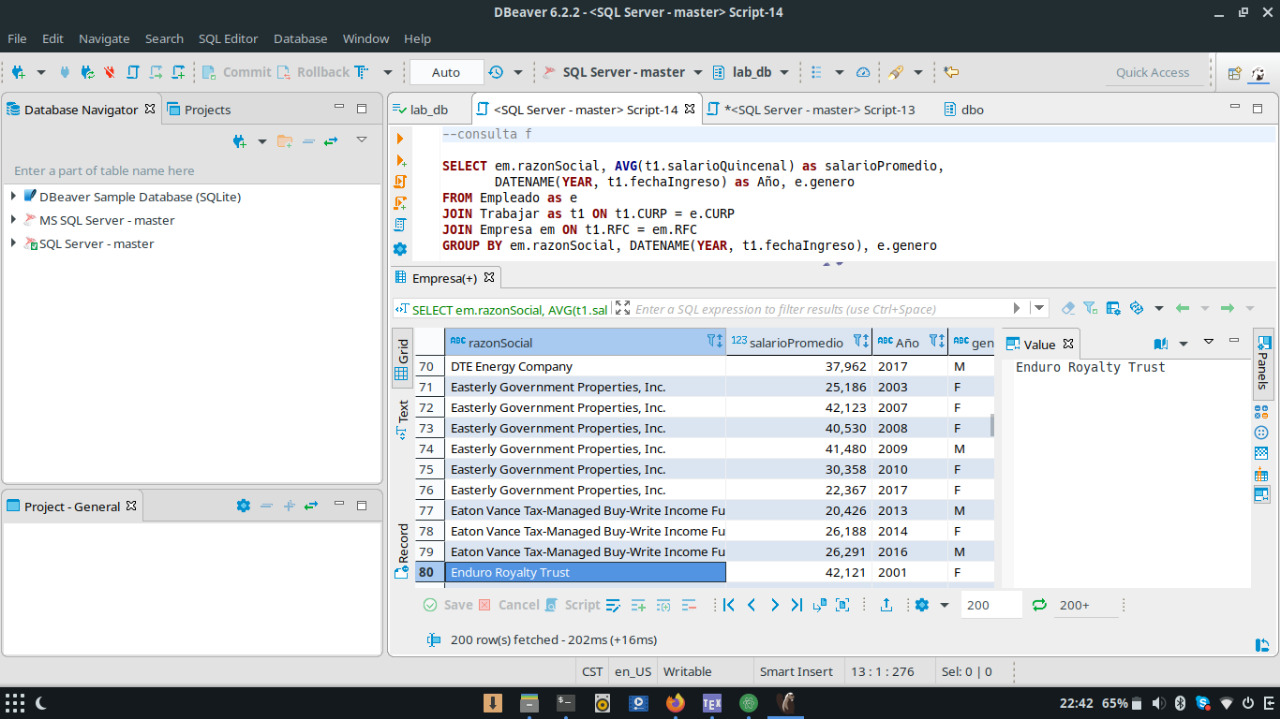
\includegraphics[width=\textwidth]
            {img/f7.jpeg}\hfill
    \caption{F 7}
    \end{figure}
    \begin{figure}
        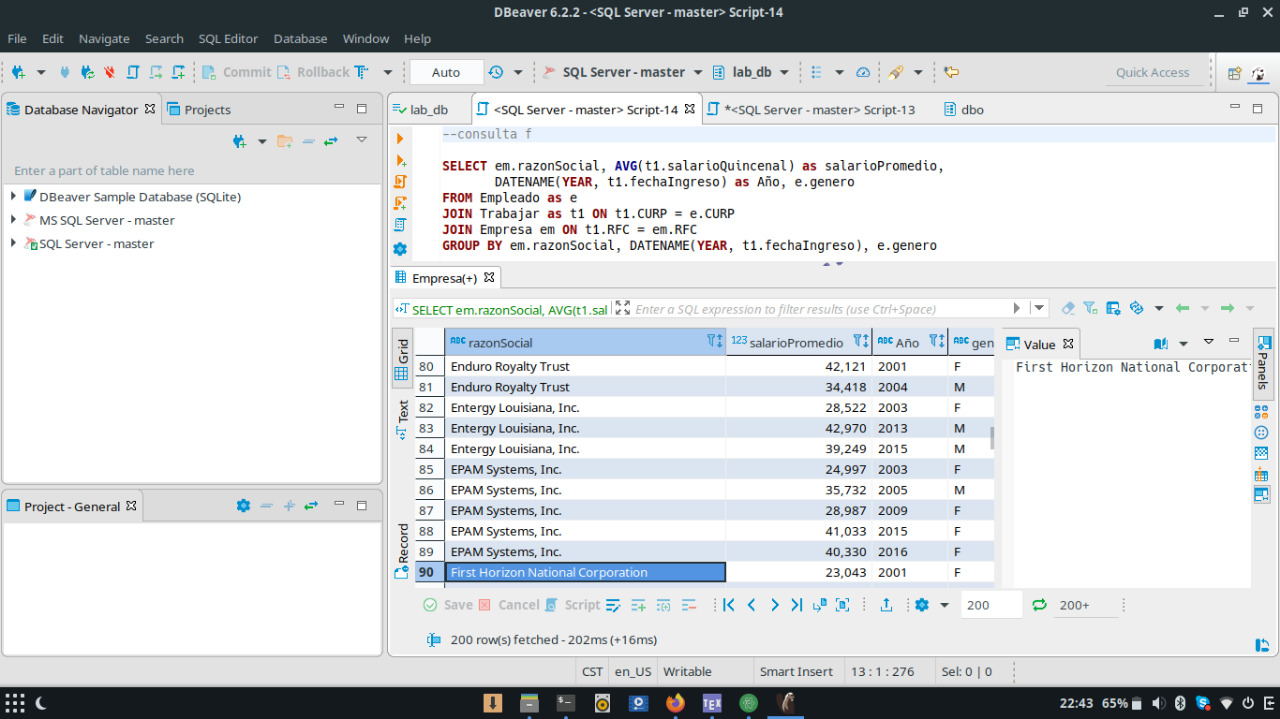
\includegraphics[width=\textwidth]
            {img/f8.jpeg}\hfill
    \caption{F 8}
    \end{figure}
    \begin{figure}
        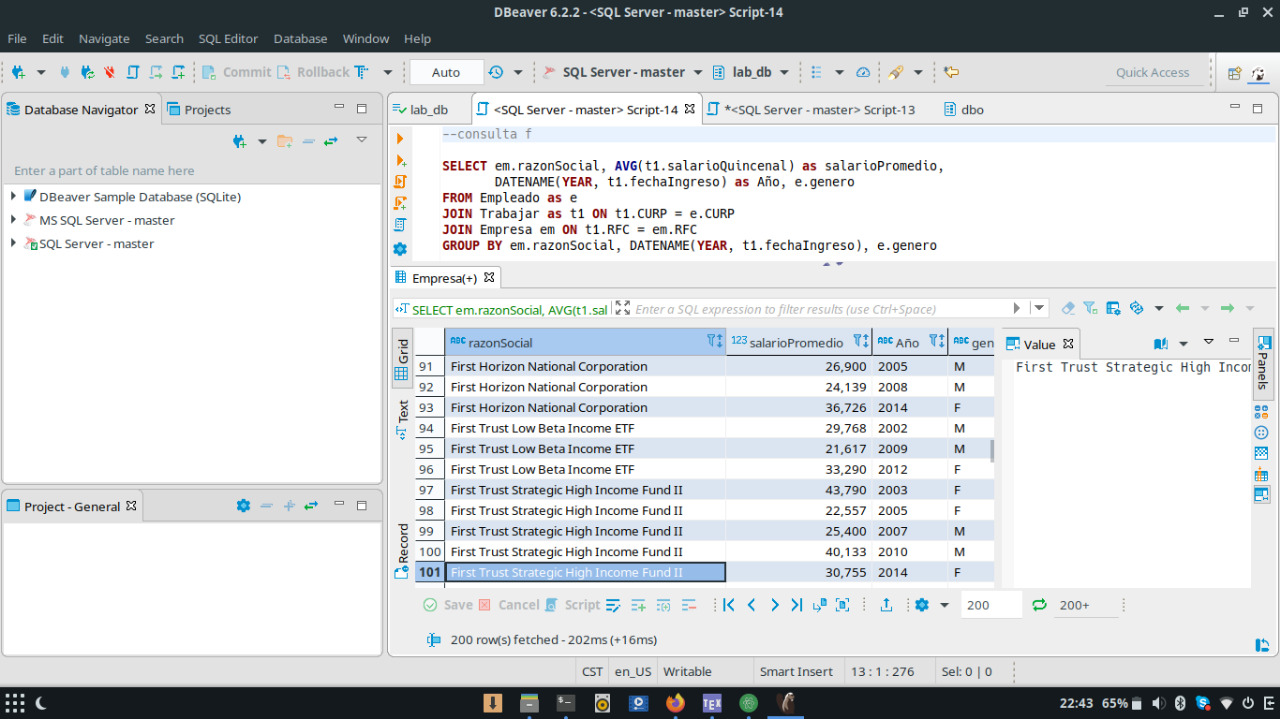
\includegraphics[width=\textwidth]
            {img/f9.jpeg}\hfill
    \caption{F 9}
    \end{figure}

\subsubsection*{Sub-inciso G}
    \begin{figure}
        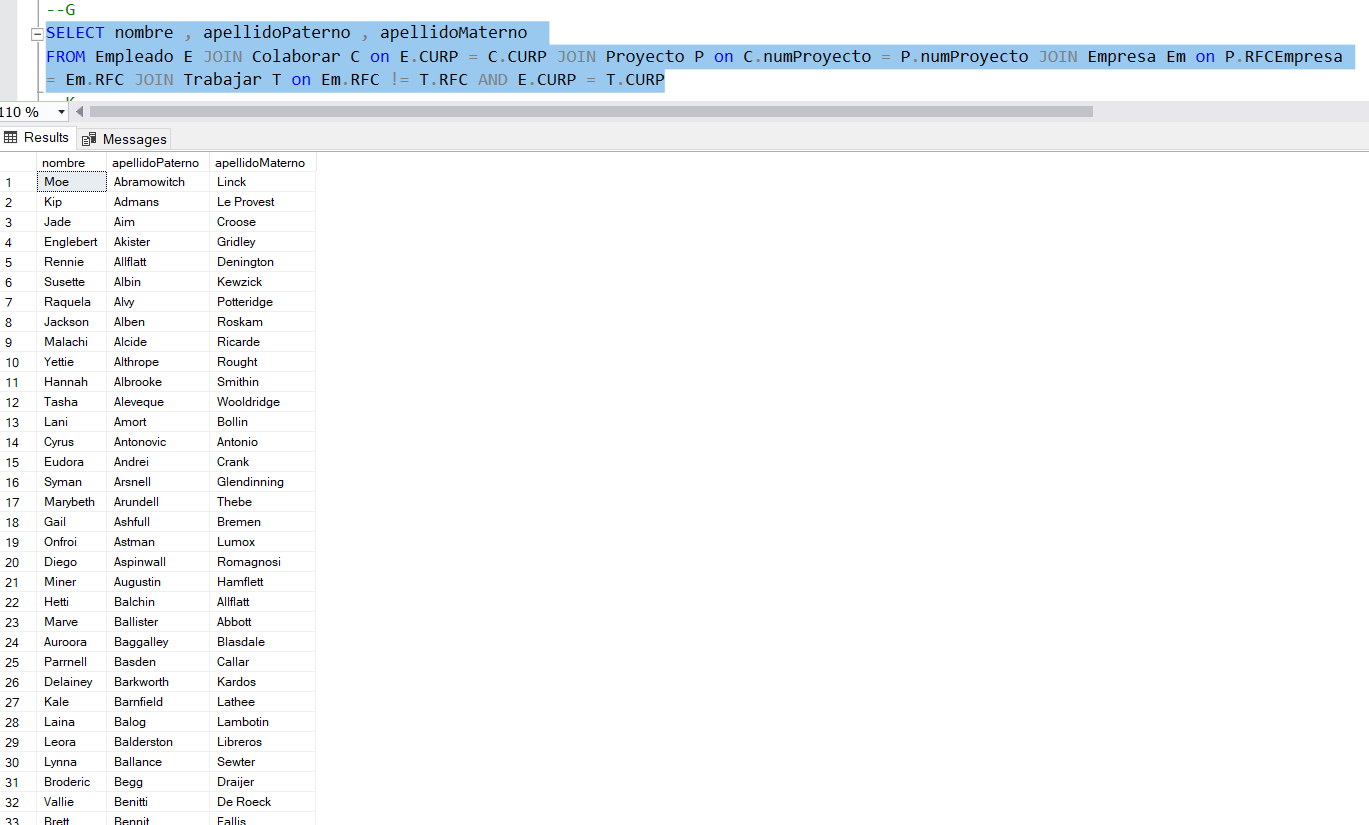
\includegraphics[width=\textwidth]
            {img/G1.png}\hfill
    \caption{G 1}
    \end{figure}
    \begin{figure}
        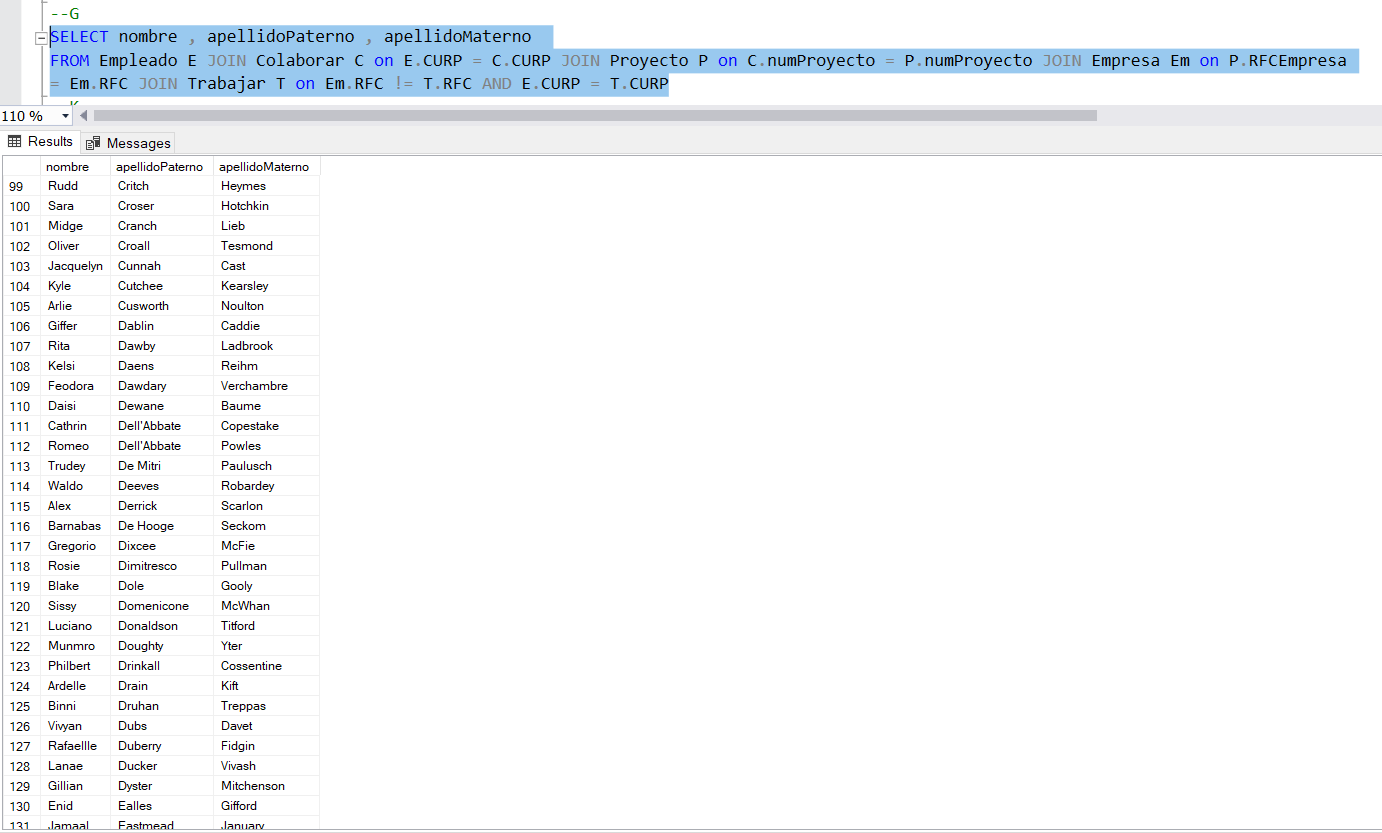
\includegraphics[width=\textwidth]
            {img/G2.png}\hfill
    \caption{G 2}
    \end{figure}
    \begin{figure}
        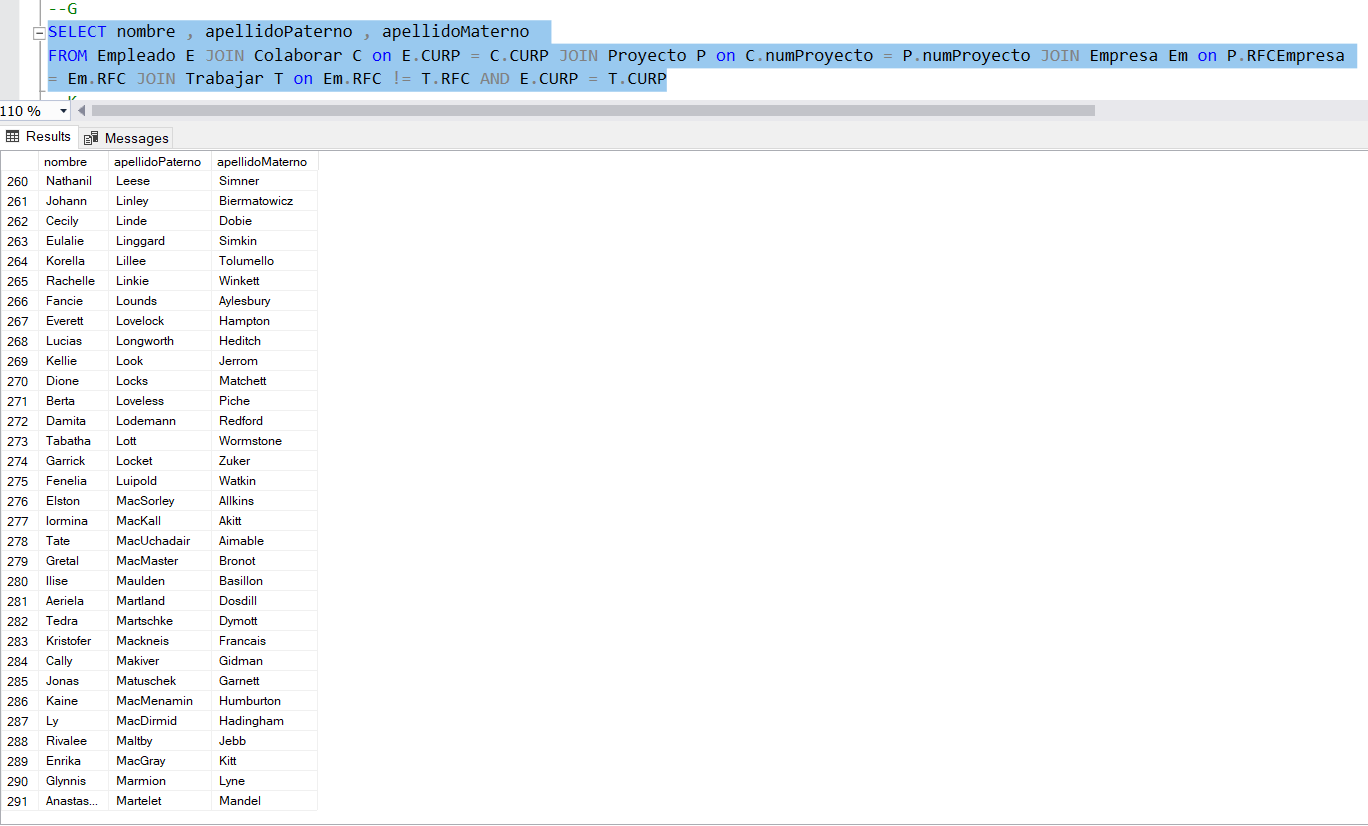
\includegraphics[width=\textwidth]
            {img/G3.png}\hfill
    \caption{G 3}
    \end{figure}

\subsubsection*{Sub-inciso H}
    \begin{figure}
        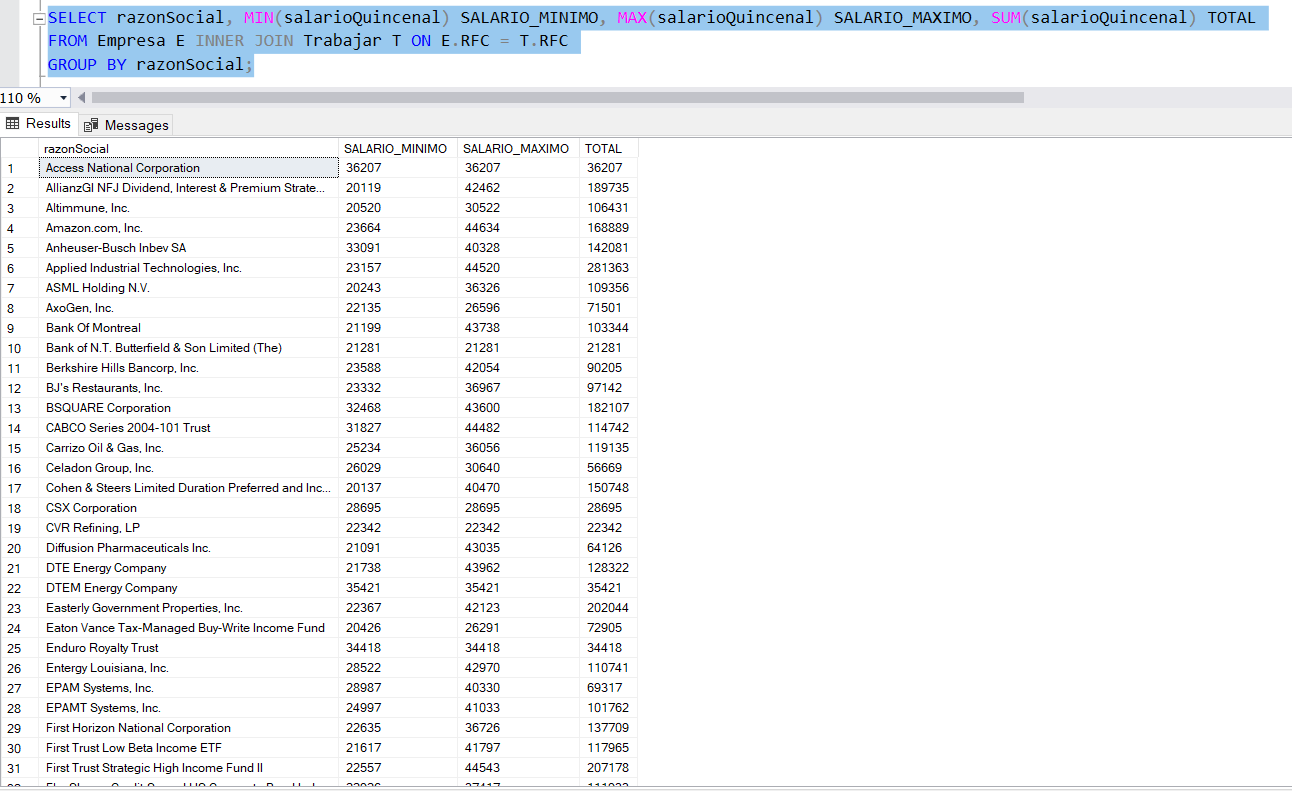
\includegraphics[width=\textwidth]
            {img/H1.png}\hfill
    \caption{H 1}
    \end{figure}
    \begin{figure}
        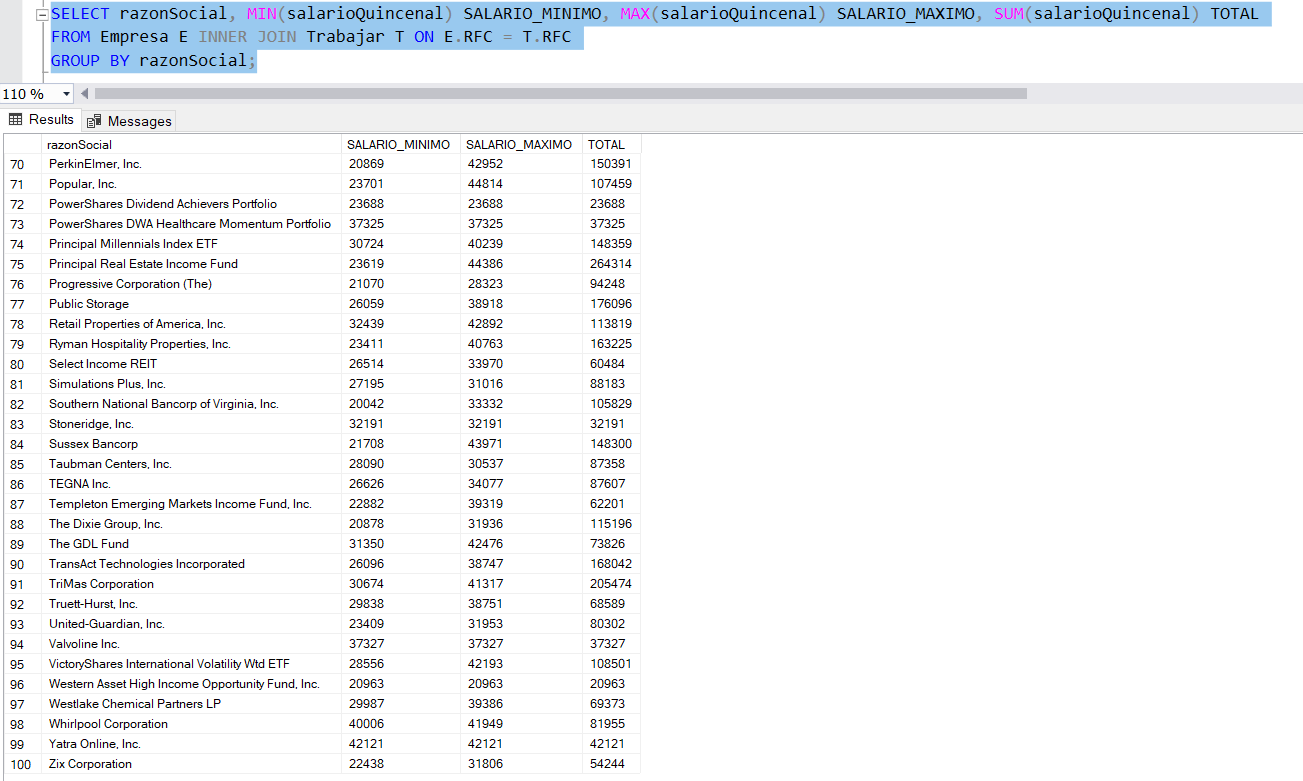
\includegraphics[width=\textwidth]
            {img/H2.png}\hfill
    \caption{H 2}
    \end{figure}

\subsubsection*{Sub-inciso I}
Ejercicio no resuelto

\subsubsection*{Sub-inciso J}
    \begin{figure}
        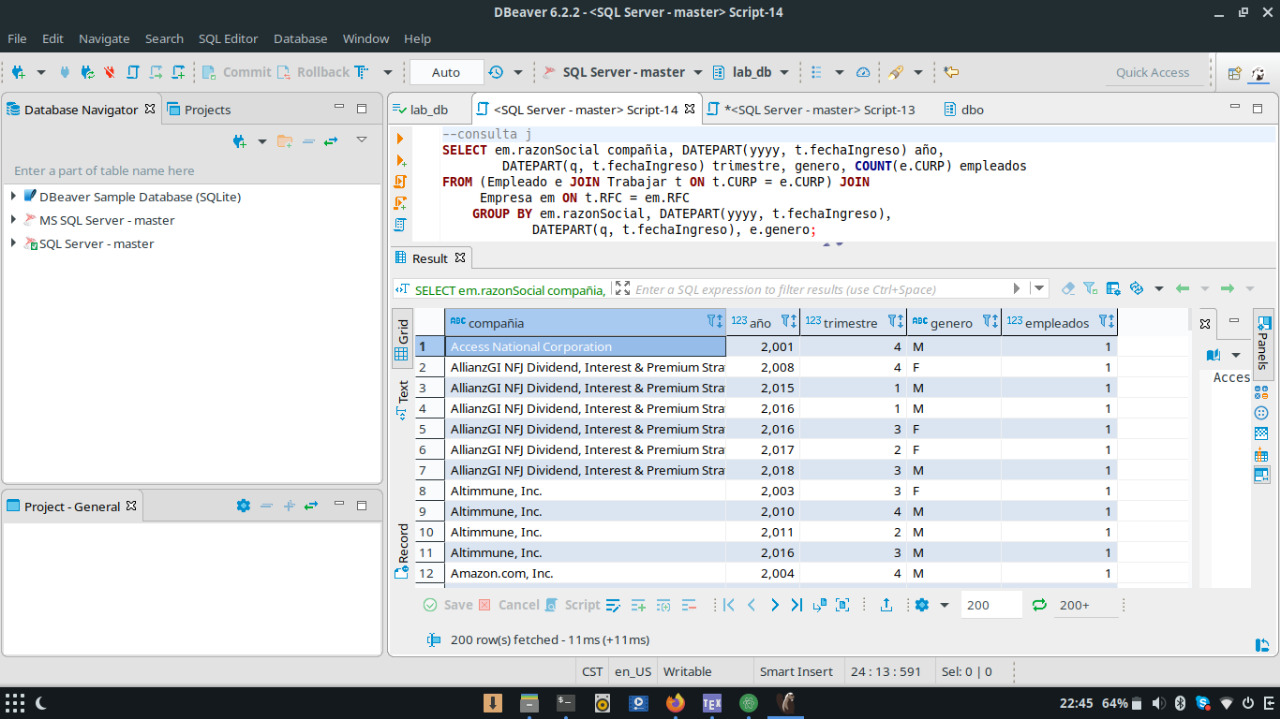
\includegraphics[width=\textwidth]
            {img/j1.jpeg}\hfill
    \caption{J 1}
    \end{figure}
    \begin{figure}
        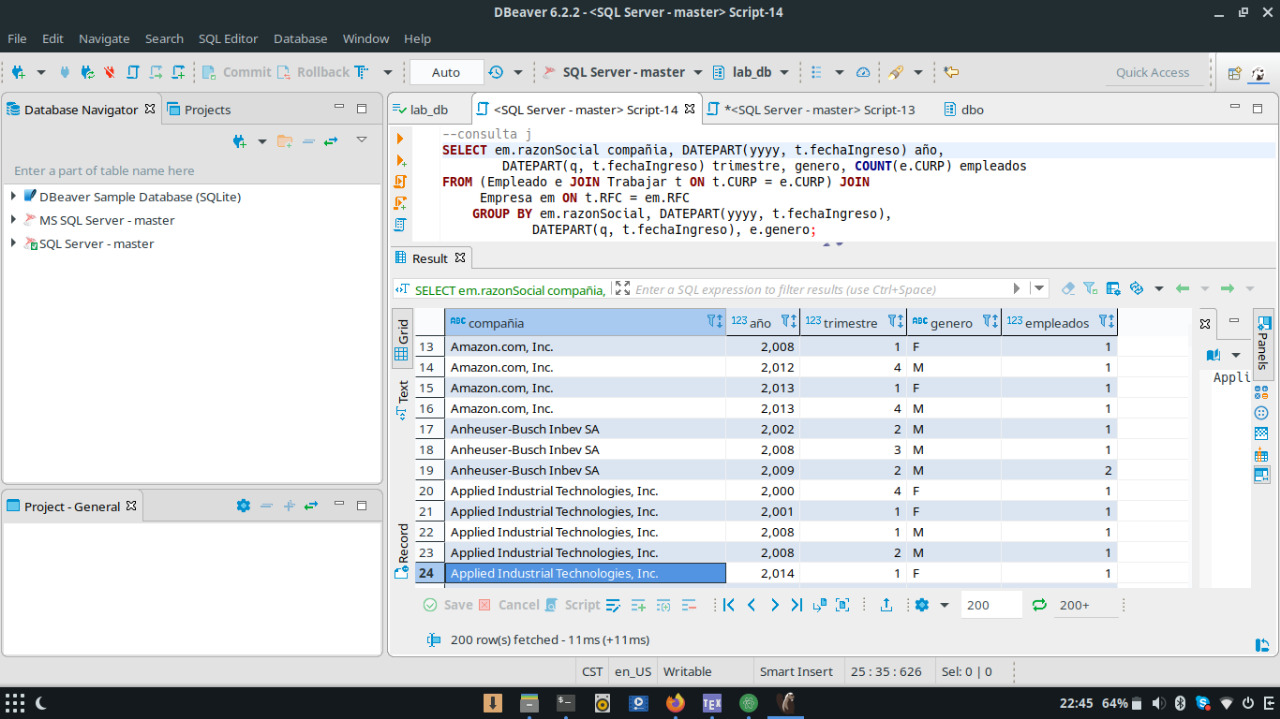
\includegraphics[width=\textwidth]
            {img/j2.jpeg}\hfill
    \caption{J 2}
    \end{figure}
    \begin{figure}
        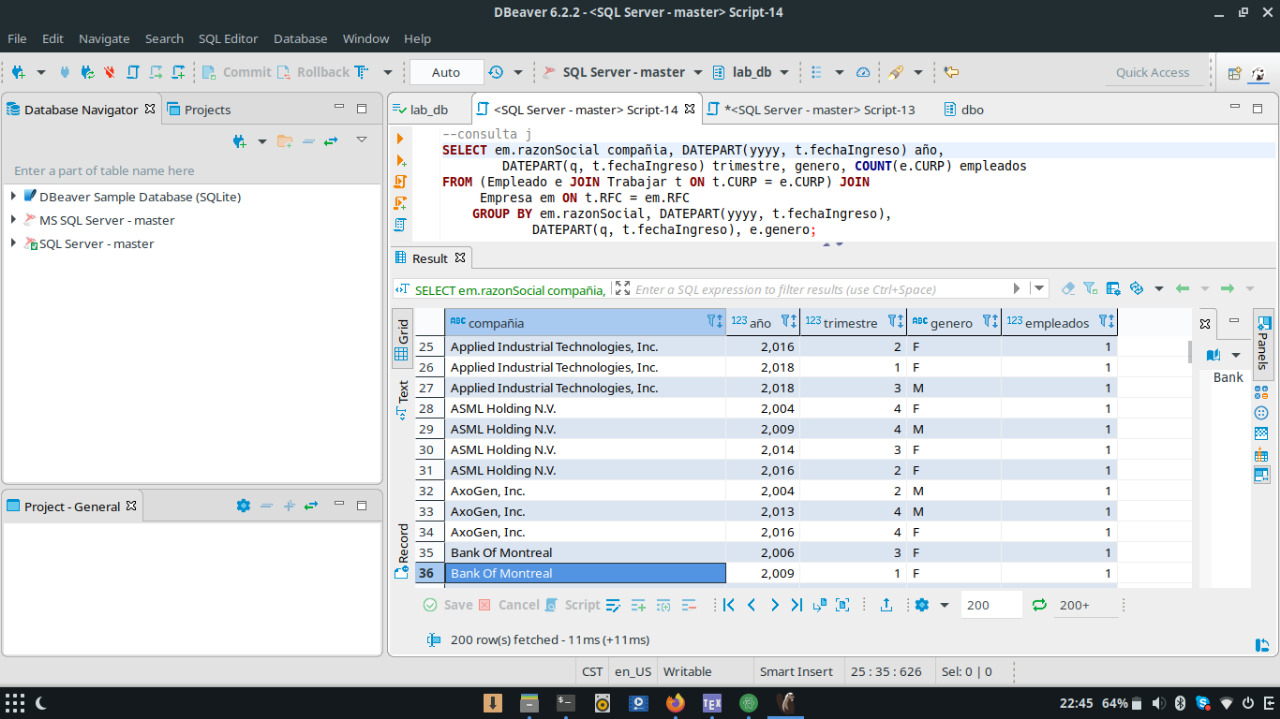
\includegraphics[width=\textwidth]
            {img/j3.jpeg}\hfill
    \caption{J 3}
    \end{figure}
    \begin{figure}
        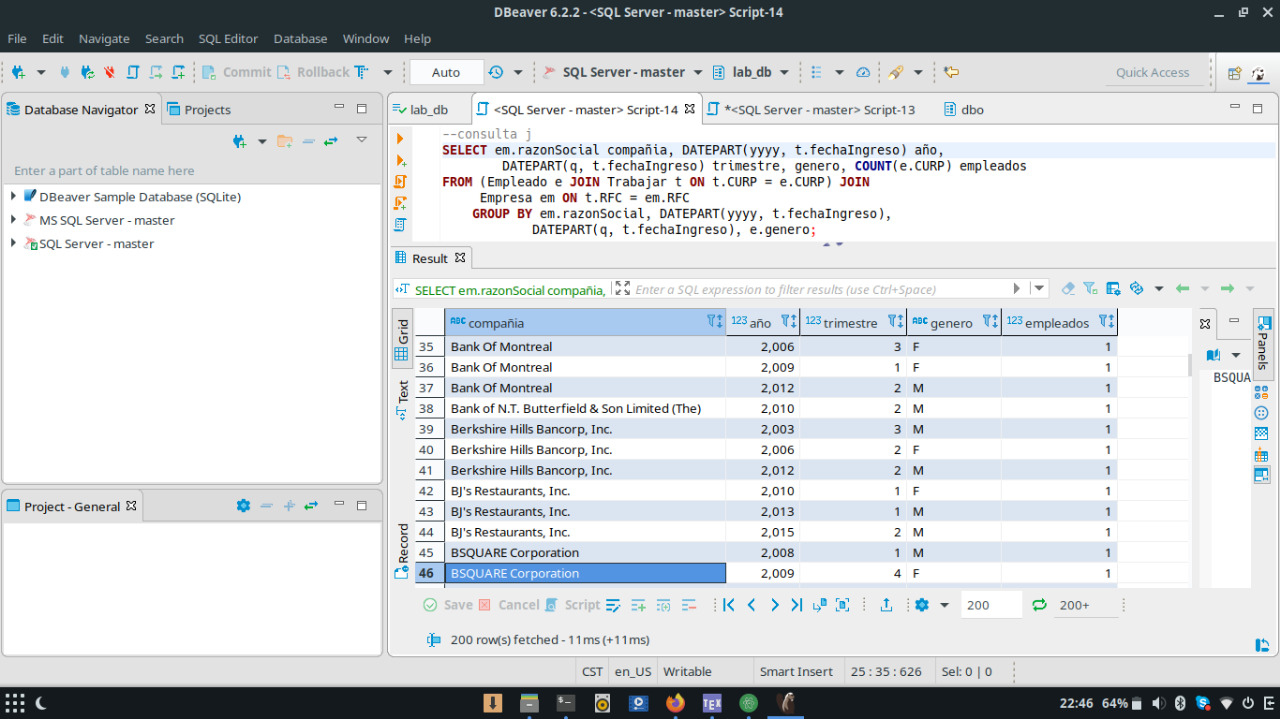
\includegraphics[width=\textwidth]
            {img/j4.jpeg}\hfill
    \caption{J 4}
    \end{figure}
    \begin{figure}
        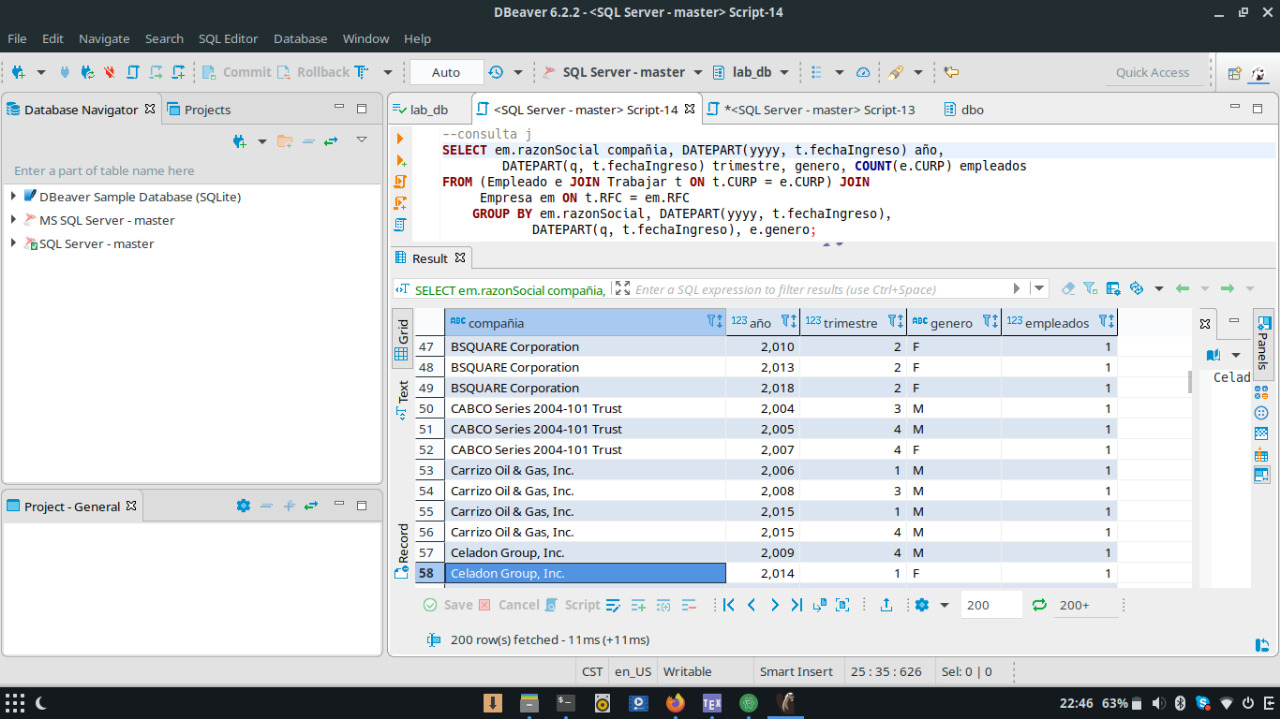
\includegraphics[width=\textwidth]
            {img/j5.jpeg}\hfill
    \caption{J 5}
    \end{figure}

\subsubsection*{Sub-inciso K}
    \begin{figure}
        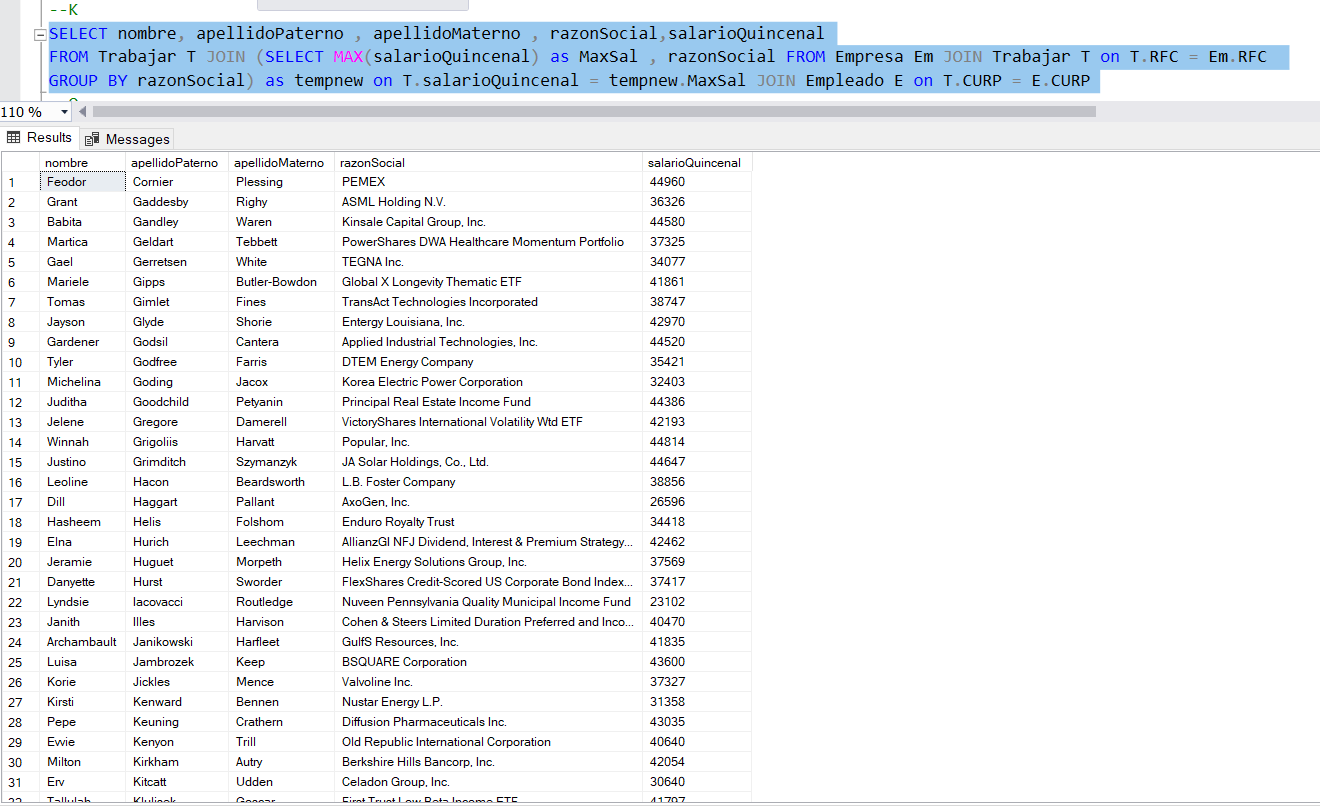
\includegraphics[width=\textwidth]
            {img/K1.png}\hfill
    \caption{K 1}
    \end{figure}
    \begin{figure}
        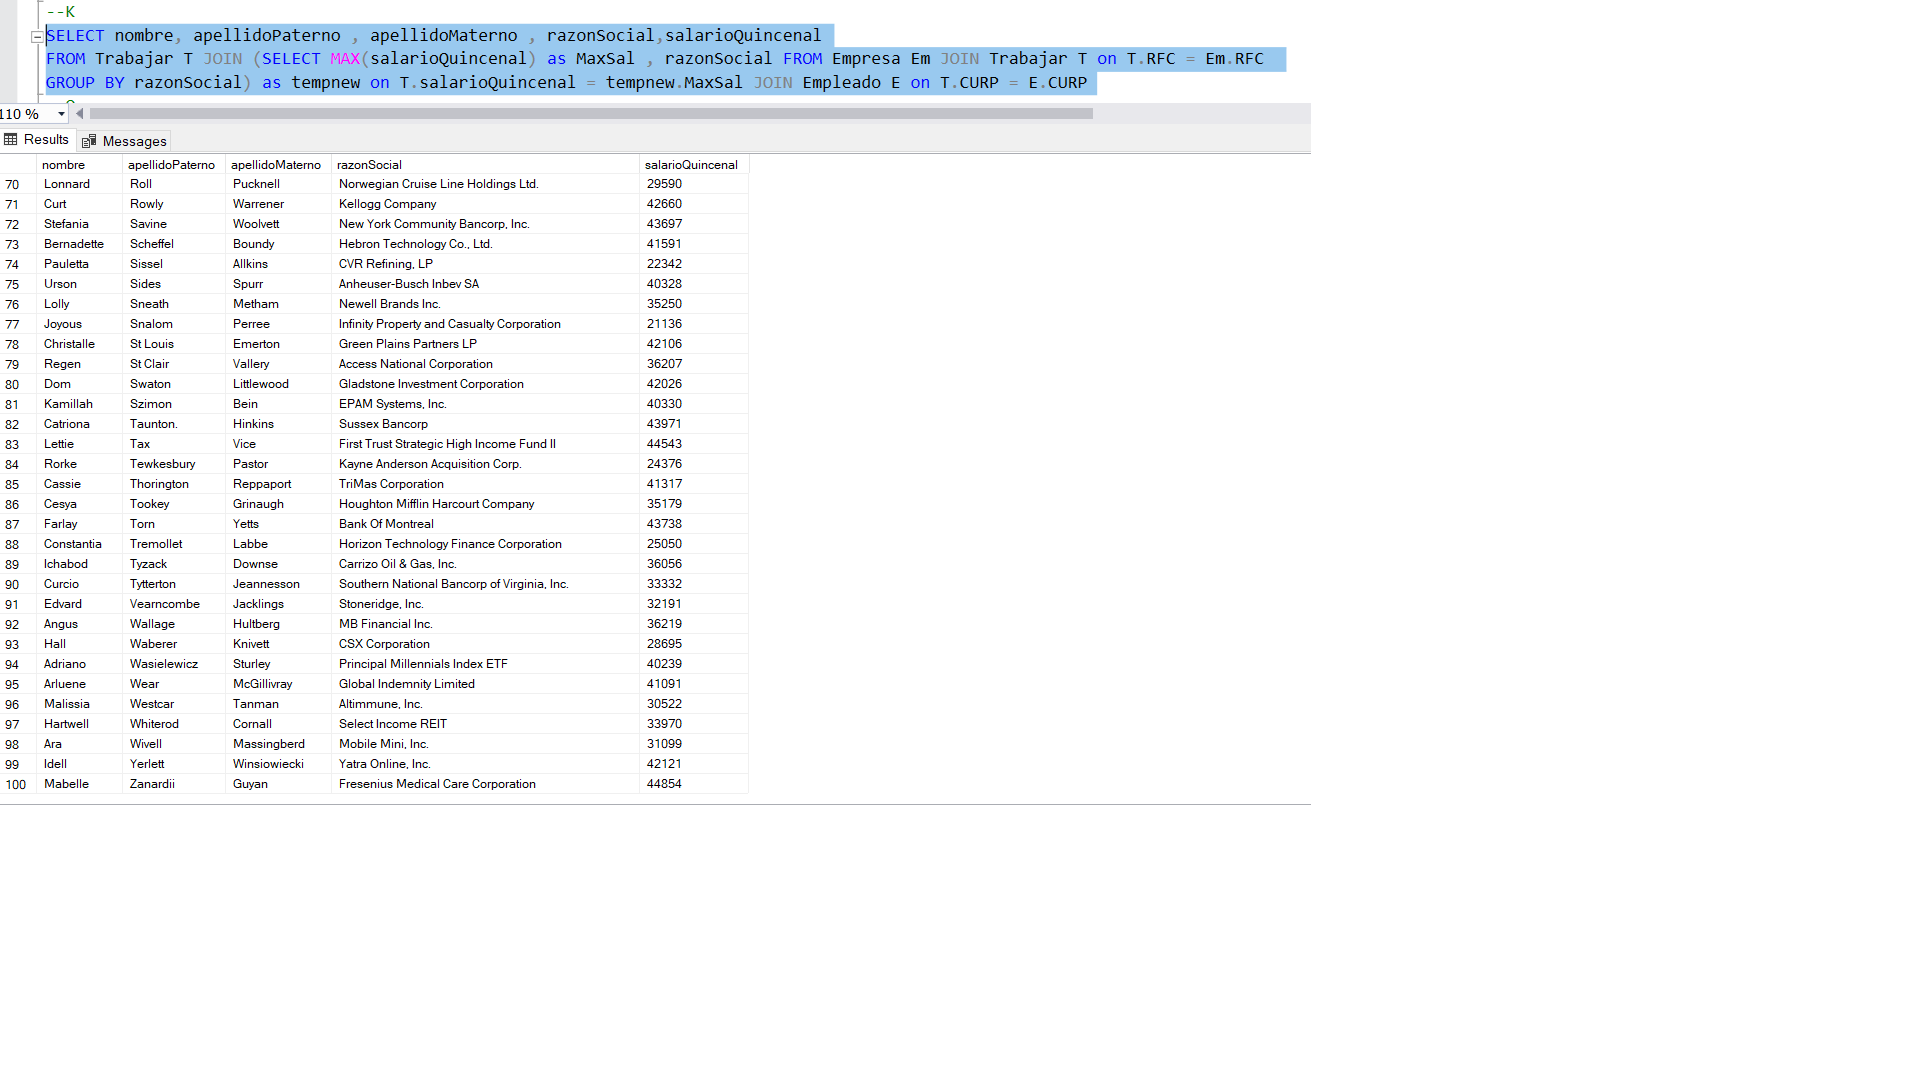
\includegraphics[width=\textwidth]
            {img/K2.png}\hfill
    \caption{K 2}
    \end{figure}

\subsubsection*{Sub-inciso L}
    \begin{figure}
        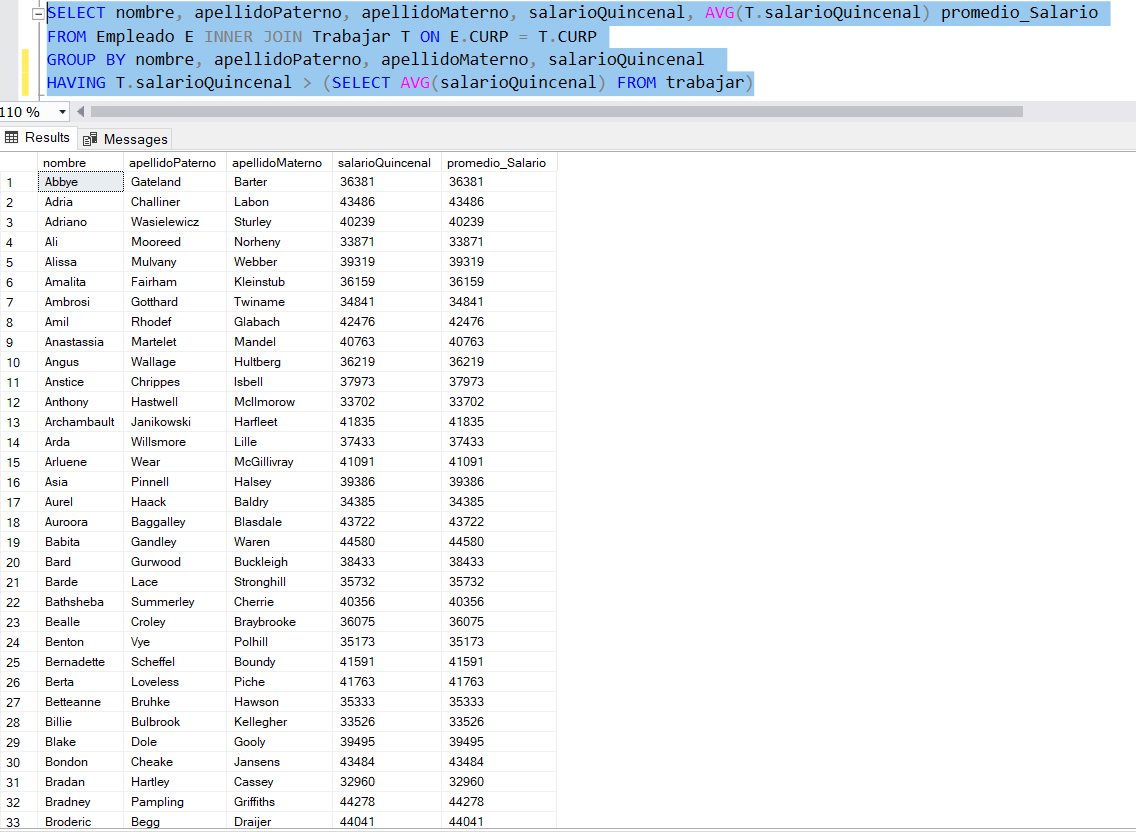
\includegraphics[width=\textwidth]
            {img/L1.png}\hfill
    \caption{L 1}
    \end{figure}
    \begin{figure}
        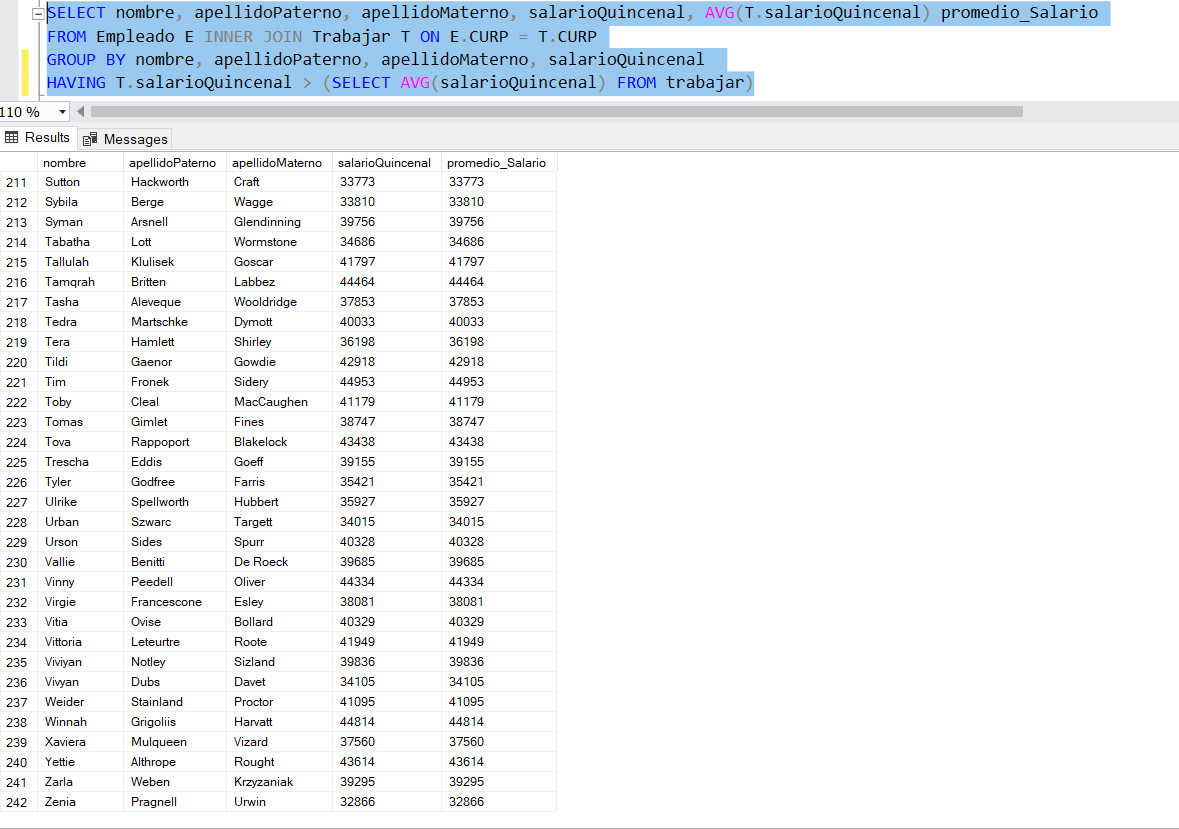
\includegraphics[width=\textwidth]
            {img/L2.png}\hfill
    \caption{L 2}
    \end{figure}

\subsubsection*{Sub-inciso M}
    \begin{figure}
        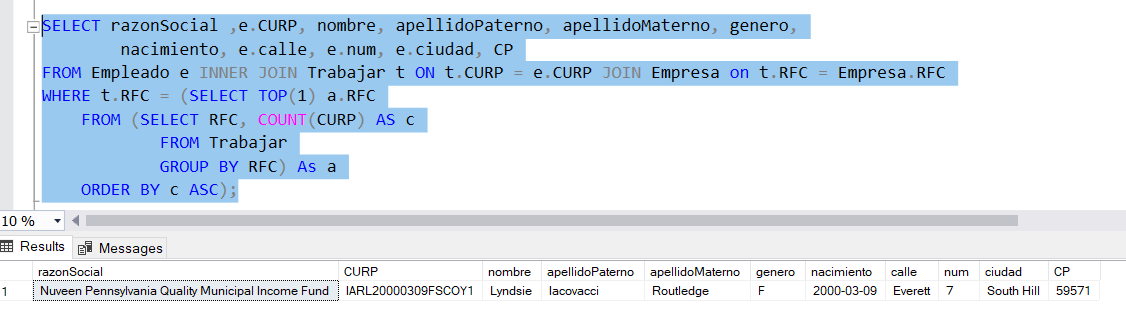
\includegraphics[width=\textwidth]
            {img/M.png}\hfill
    \caption{M}
    \end{figure}

\subsubsection*{Sub-inciso N}
    \begin{figure}
        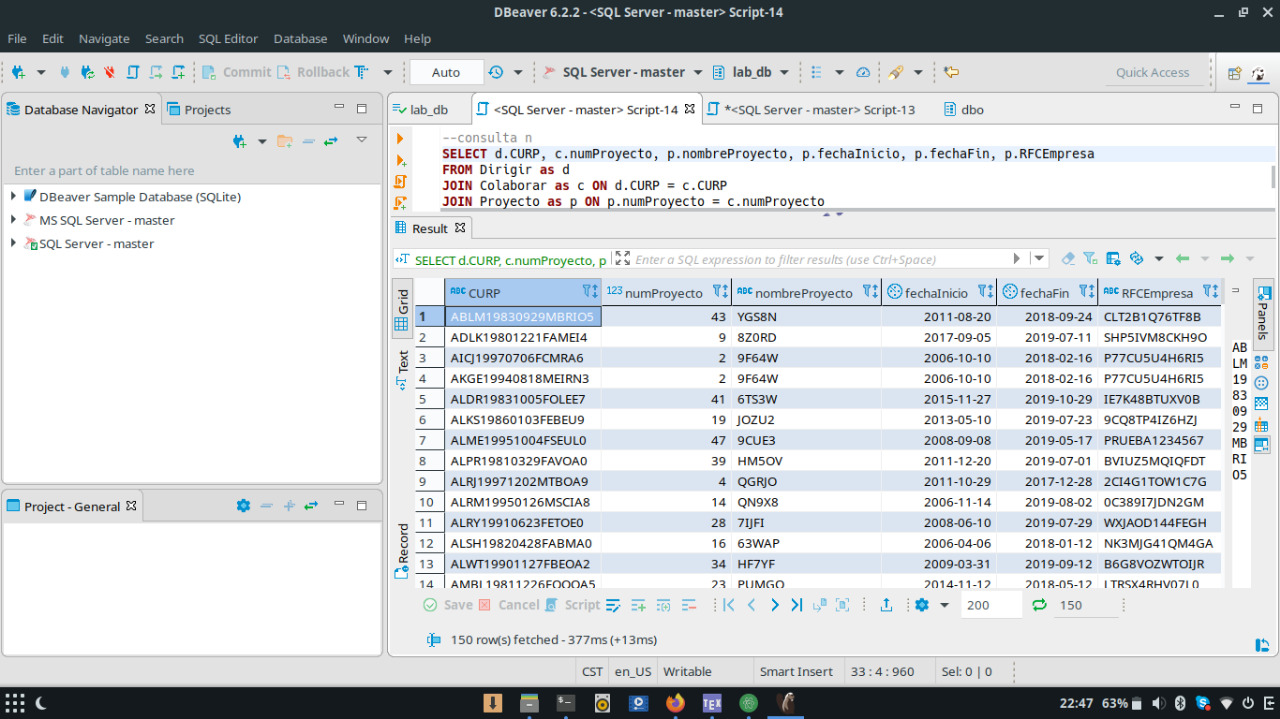
\includegraphics[width=\textwidth]
            {img/n1.jpeg}\hfill
    \caption{N 1}
    \end{figure}
    \begin{figure}
        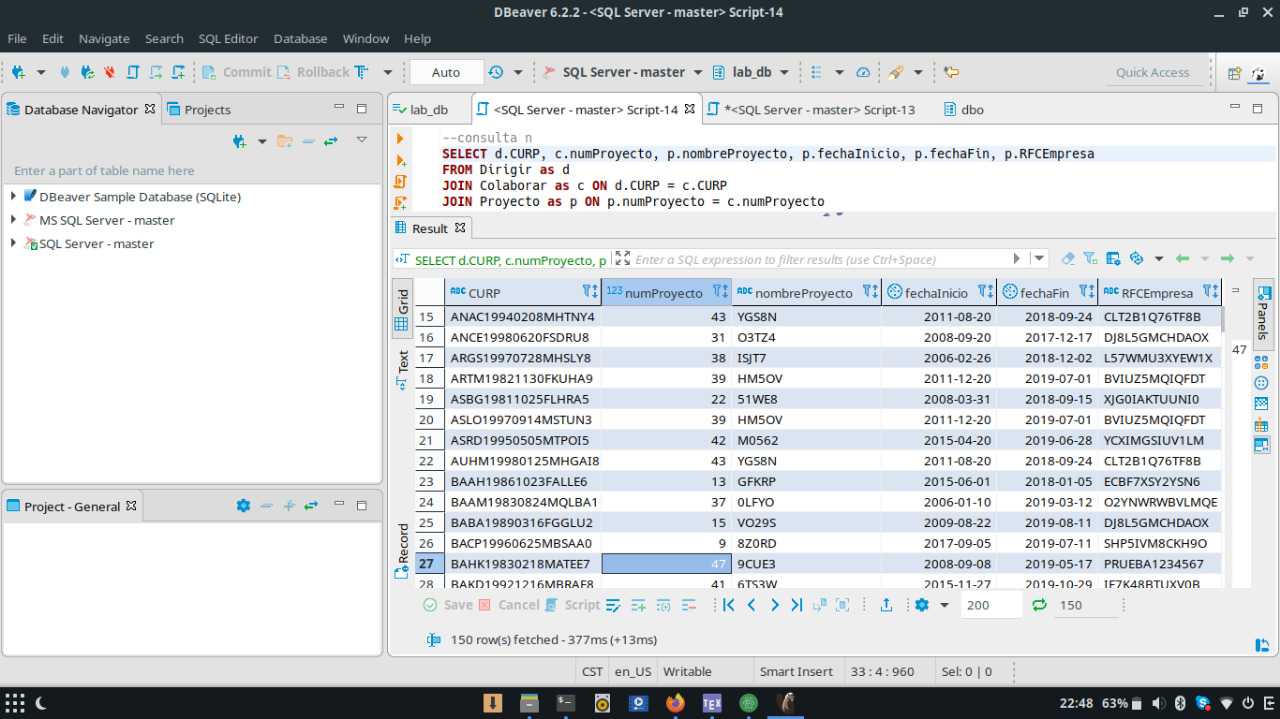
\includegraphics[width=\textwidth]
            {img/n2.jpeg}\hfill
    \caption{N 2}
    \end{figure}
    \begin{figure}
        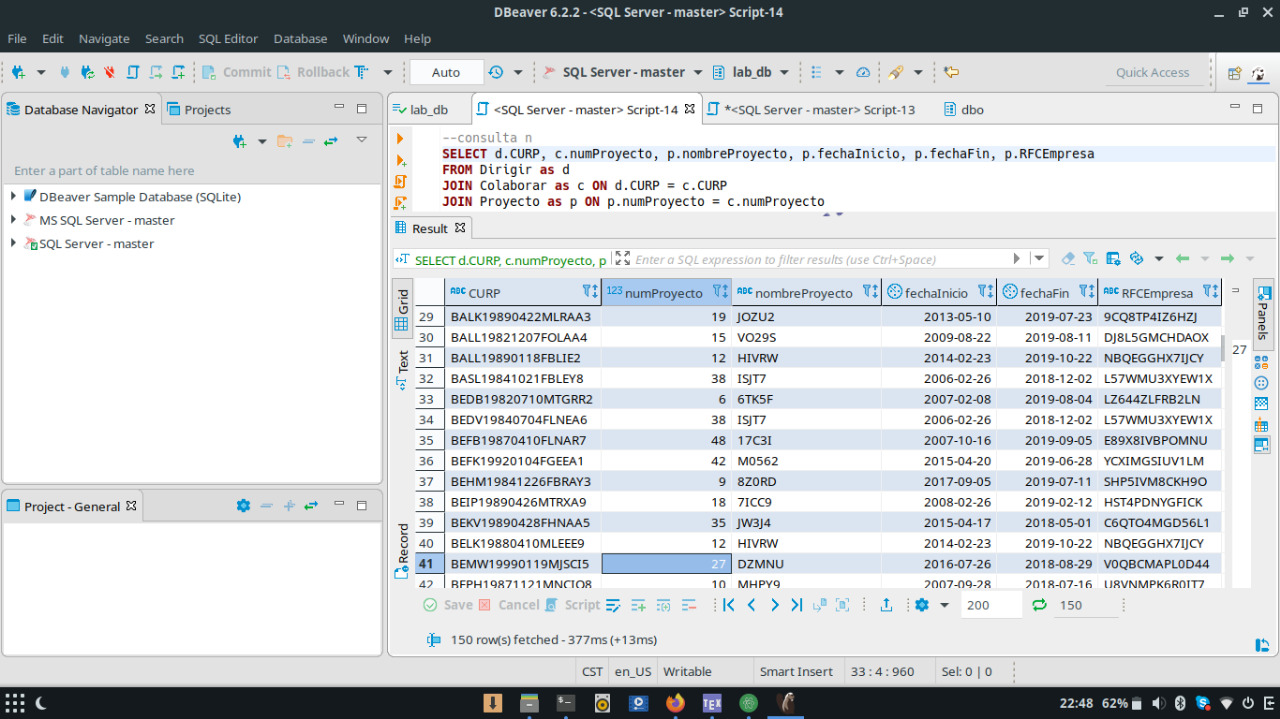
\includegraphics[width=\textwidth]
            {img/n3.jpeg}\hfill
    \caption{N 3}
    \end{figure}
    \begin{figure}
        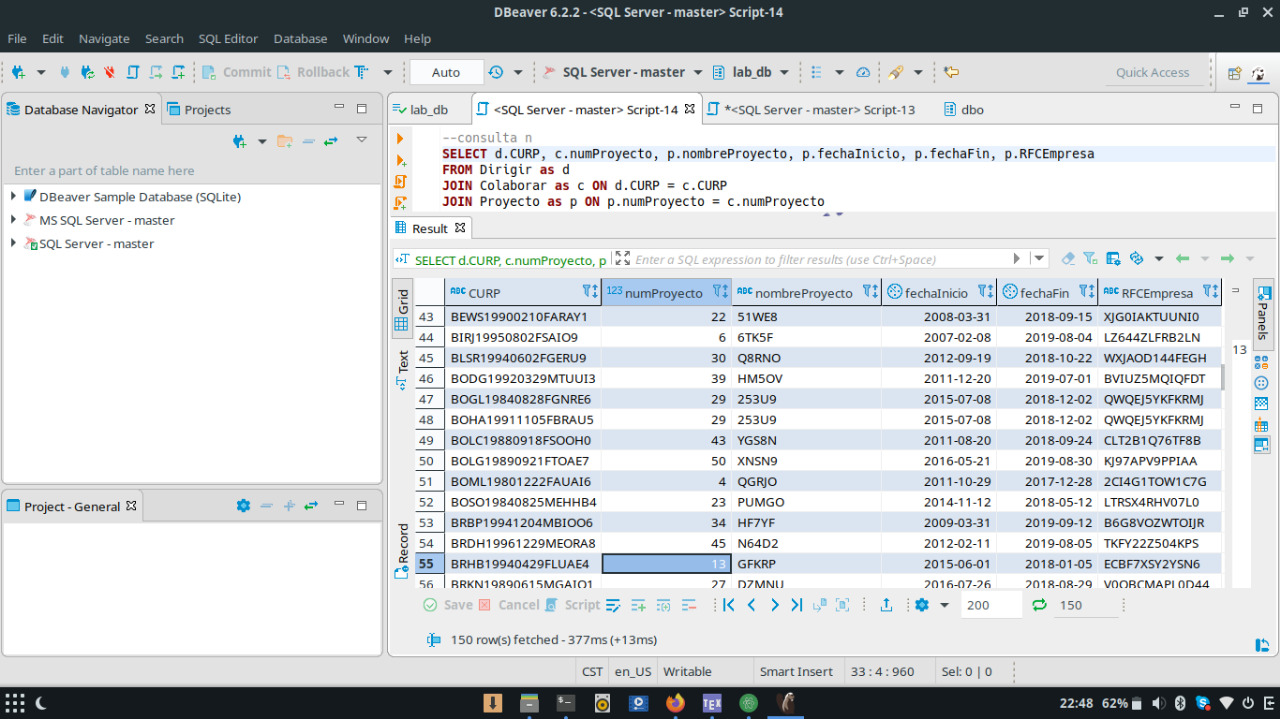
\includegraphics[width=\textwidth]
            {img/n4.jpeg}\hfill
    \caption{N 4}
    \end{figure}

\subsubsection*{Sub-inciso O}
    \begin{figure}
        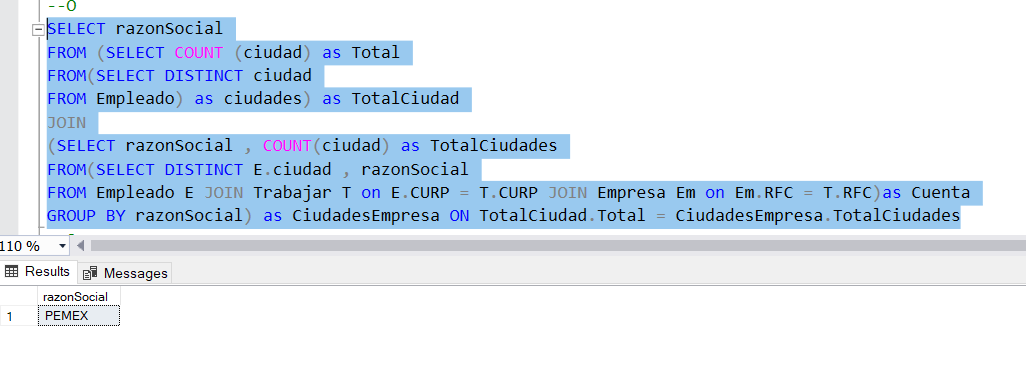
\includegraphics[width=\textwidth]
            {img/O.png}\hfill
    \caption{O}
    \end{figure}

\subsubsection*{Sub-inciso P}
    \begin{figure}
        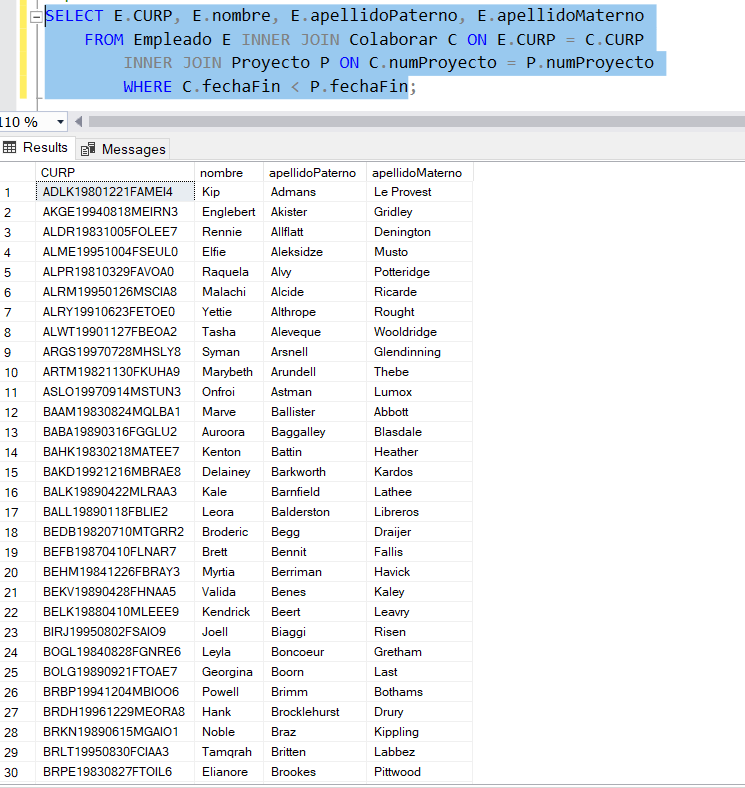
\includegraphics[width=\textwidth]
            {img/P.png}\hfill
    \caption{P 1}
    \end{figure}
    \begin{figure}
        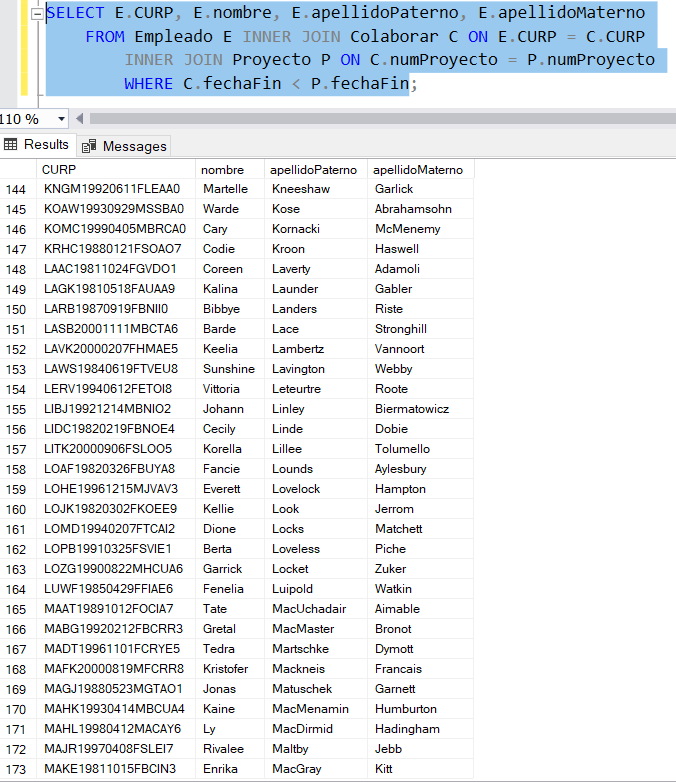
\includegraphics[width=\textwidth]
            {img/P2.png}\hfill
    \caption{P 2}
    \end{figure}

\subsubsection*{Sub-inciso Q}
    \begin{figure}
        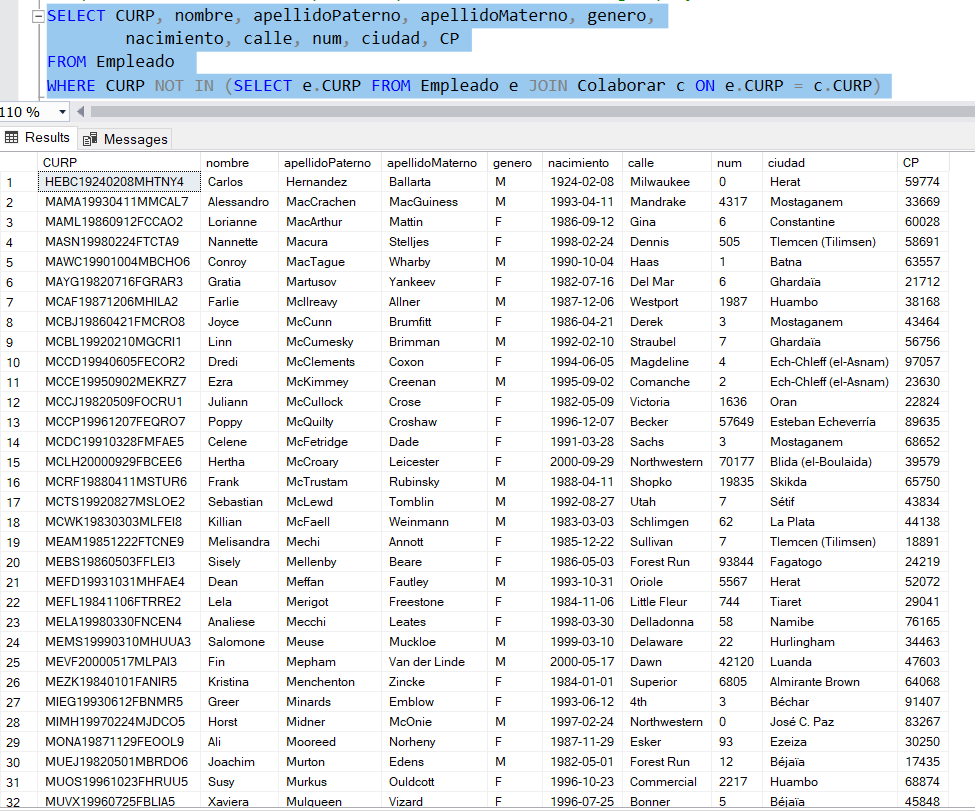
\includegraphics[width=\textwidth]
            {img/Q1.png}\hfill
    \caption{Q 1}
    \end{figure}
    \begin{figure}
        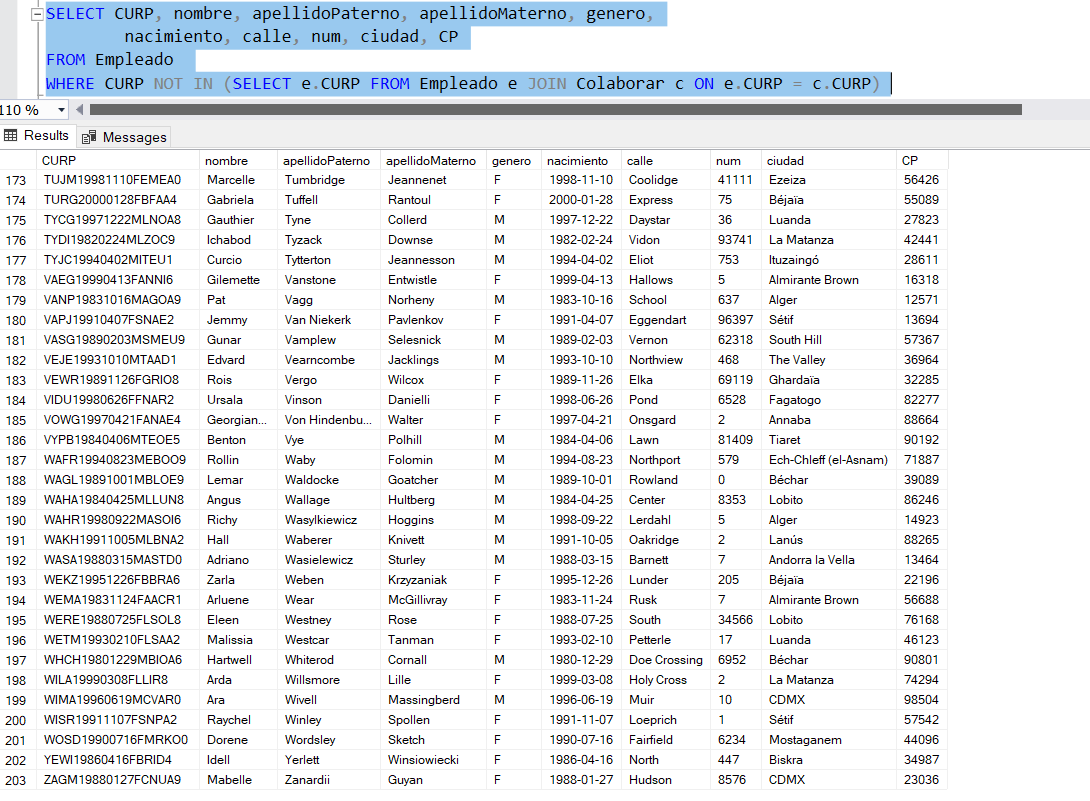
\includegraphics[width=\textwidth]
            {img/Q2.png}\hfill
    \caption{Q 2}
    \end{figure}

\subsubsection*{Sub-inciso R}
    \begin{figure}
        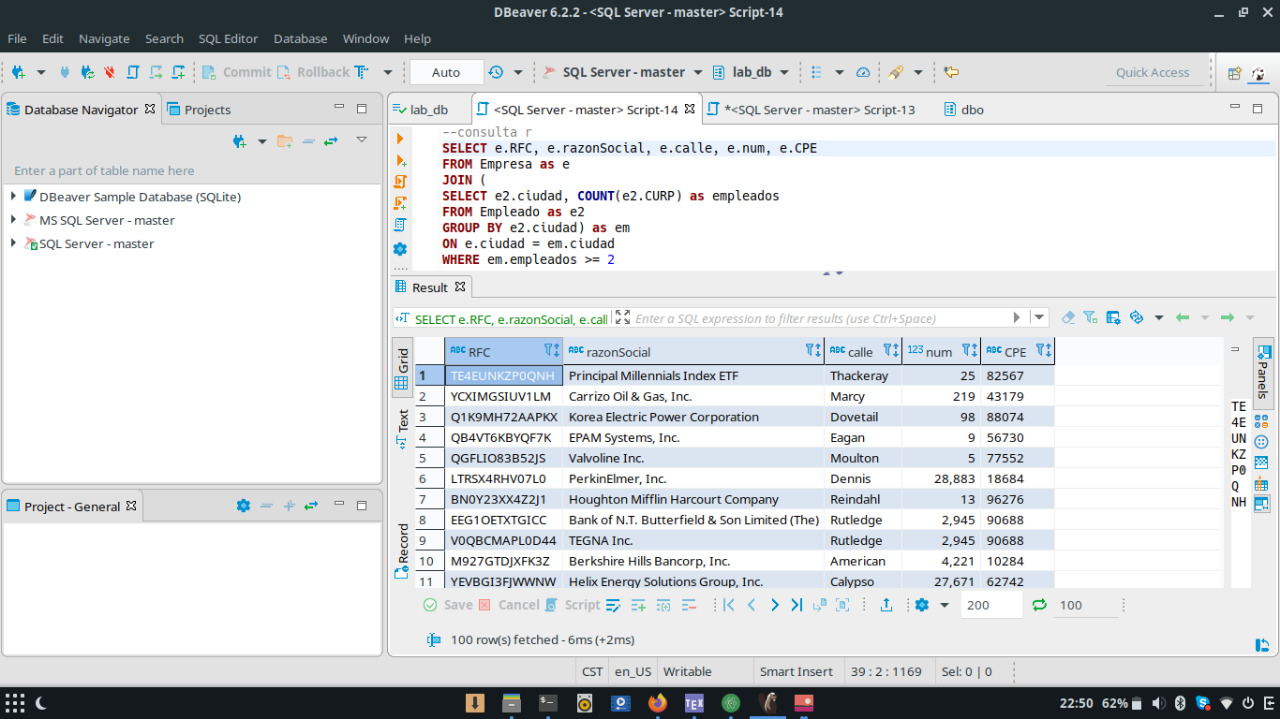
\includegraphics[width=\textwidth]
            {img/r1.jpeg}\hfill
    \caption{R 1}
    \end{figure}
    \begin{figure}
        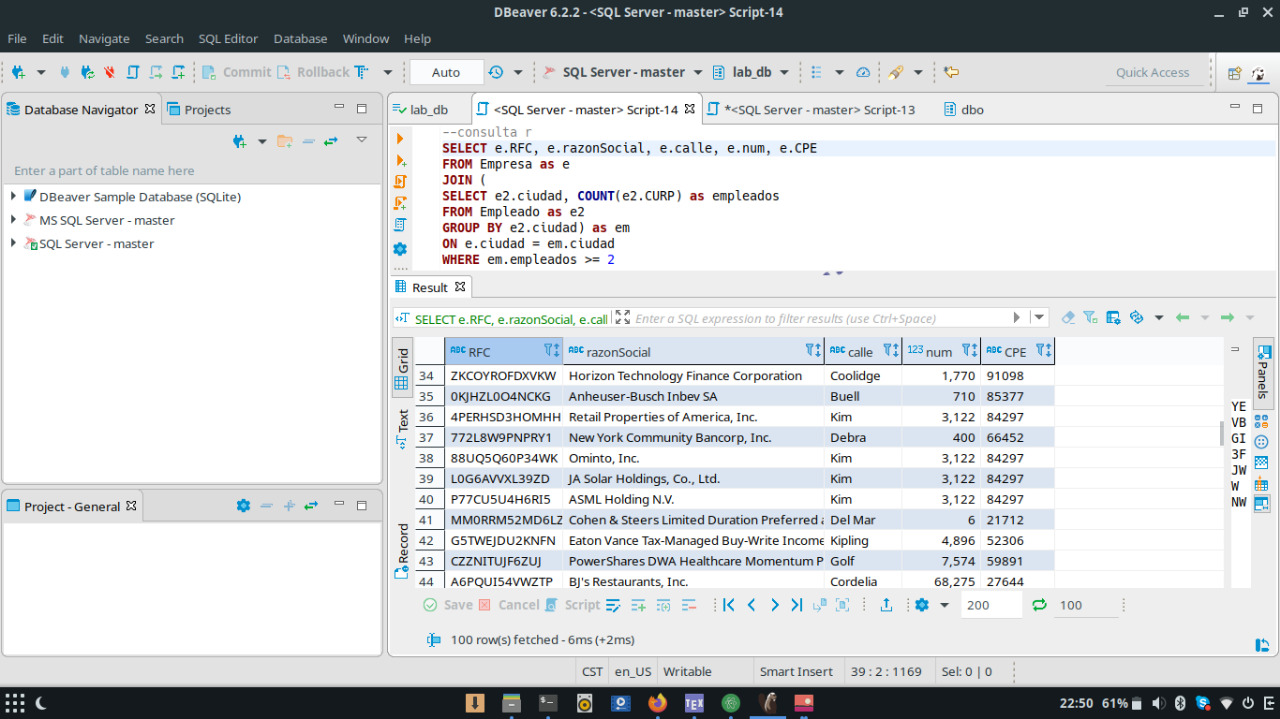
\includegraphics[width=\textwidth]
            {img/r2.jpeg}\hfill
    \caption{R 2}
    \end{figure}
    \begin{figure}
        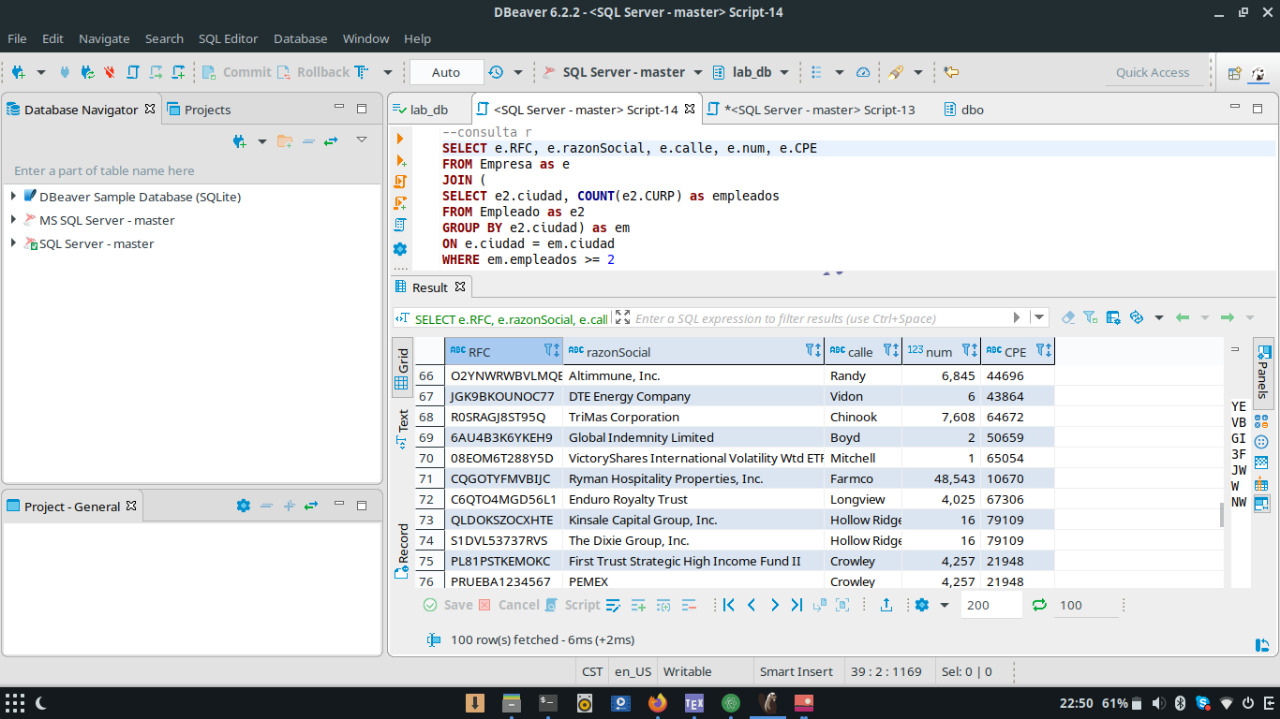
\includegraphics[width=\textwidth]
            {img/r3.jpeg}\hfill
    \caption{R 3}
    \end{figure}
    \begin{figure}
        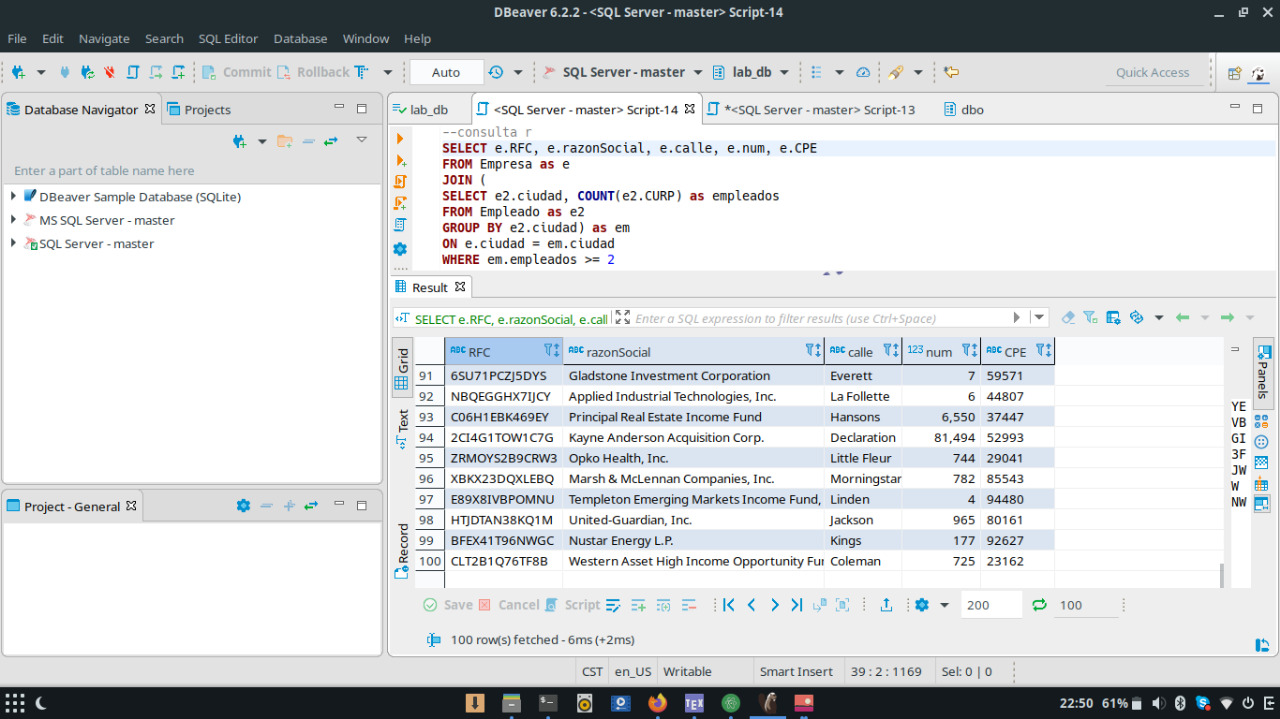
\includegraphics[width=\textwidth]
            {img/r4.jpeg}\hfill
    \caption{R 4}
    \end{figure}

\subsubsection*{Sub-inciso S}
    \begin{figure}
        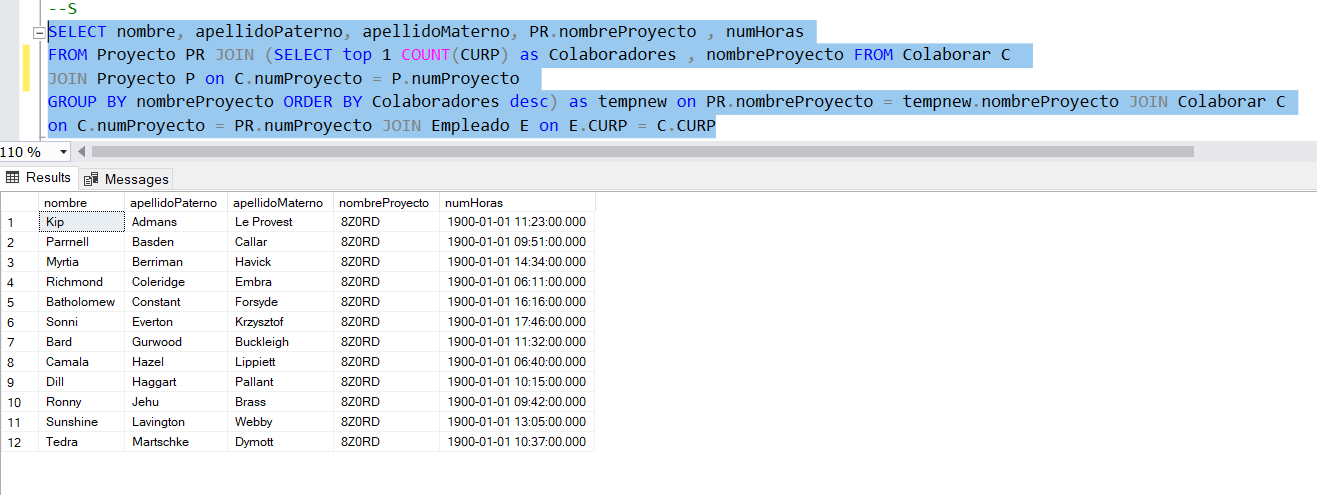
\includegraphics[width=\textwidth]
            {img/S.png}\hfill
    \caption{S}
    \end{figure}

\subsubsection*{Sub-inciso T}
    \begin{figure}
        \includegraphics[width=\textwidth]
            {img/T.png}\hfill
    \caption{T}
    \end{figure}

\subsubsection*{Sub-inciso U}
    \begin{figure}
        \includegraphics[width=\textwidth]
            {img/U1.png}\hfill
    \caption{U 1}
    \end{figure}
    \begin{figure}
        \includegraphics[width=\textwidth]
            {img/U2.png}\hfill
    \caption{U 2}
    \end{figure}

\subsubsection*{Sub-inciso V}
    \begin{figure}
        \includegraphics[width=\textwidth]
            {img/V.png}\hfill
    \caption{V}
    \end{figure}

\subsubsection*{Sub-inciso W}
    \begin{figure}
        \includegraphics[width=\textwidth]
            {img/W1.png}\hfill
    \caption{W 1}
    \end{figure}
    \begin{figure}
        \includegraphics[width=\textwidth]
            {img/W2.png}\hfill
    \caption{W 2}
    \end{figure}

\subsubsection*{Sub-inciso X}
    \begin{figure}
        \includegraphics[width=\textwidth]
            {img/X.png}\hfill
    \caption{X}
    \end{figure}

\subsection*{Inciso 5}
Las ventajas incluyen dar consistencia a los datos al asegurar que cierto valor
tiene que estar en la base de datos.\\
Cómo desventaja tenemos que al momento de poblar la base, si alguna de estas
restricciones no se cumplen entonces no van a poder ser ingresados los datos.
\end{document}
